\chapter{Método de trabajo}
\label{chap:metodo}

\drop{A}{} lo largo de este capítulo se presenta la metodología de desarrollo empleada durante el ciclo de vida del proyecto, analizando las diferentes etapas e iteraciones por las que ha pasado el mismo. Además se detallan los diferentes entregables producidos durante el proceso de desarrollo.

En primer lugar se presenta una visión global sobre el proceso de desarrollo, así como algunos detalles sobre las etapas e iteraciones por las que ha pasado el desarrollo del proyecto. En segundo lugar se estudia el análisis de requisitos del sistema, haciendo énfasis en aspectos como la calidad y la evolución, y no sólo en la funcionalidad. Después se ofrece un estudio detallado sobre los casos de uso del sistema, para dar paso al diseño e implementación del mismo. En la sección \ref{sec::implementacion} se hará también un repaso por las tecnologías empleadas para implementar BreakBrain. Por último se presentará la documentación de pruebas.

\section{Proceso Unificado de Desarrollo}
\label{sec::pud}

Para este proyecto se ha seguido una metodología de desarrollo iterativa, basada en el \ac{PUD} ---también conocido como \ac{RUP}---. Se trata de un \emph{``Proceso de Ingeniería del Software''}, según \cite{Rational1998}. Su meta es asegurar la producción de software de alta calidad, satisfaciendo las necesidades del usuario final y acotando la planificación y el presupuesto de una forma predecible.

\begin{figure}[h]
  \begin{center}
    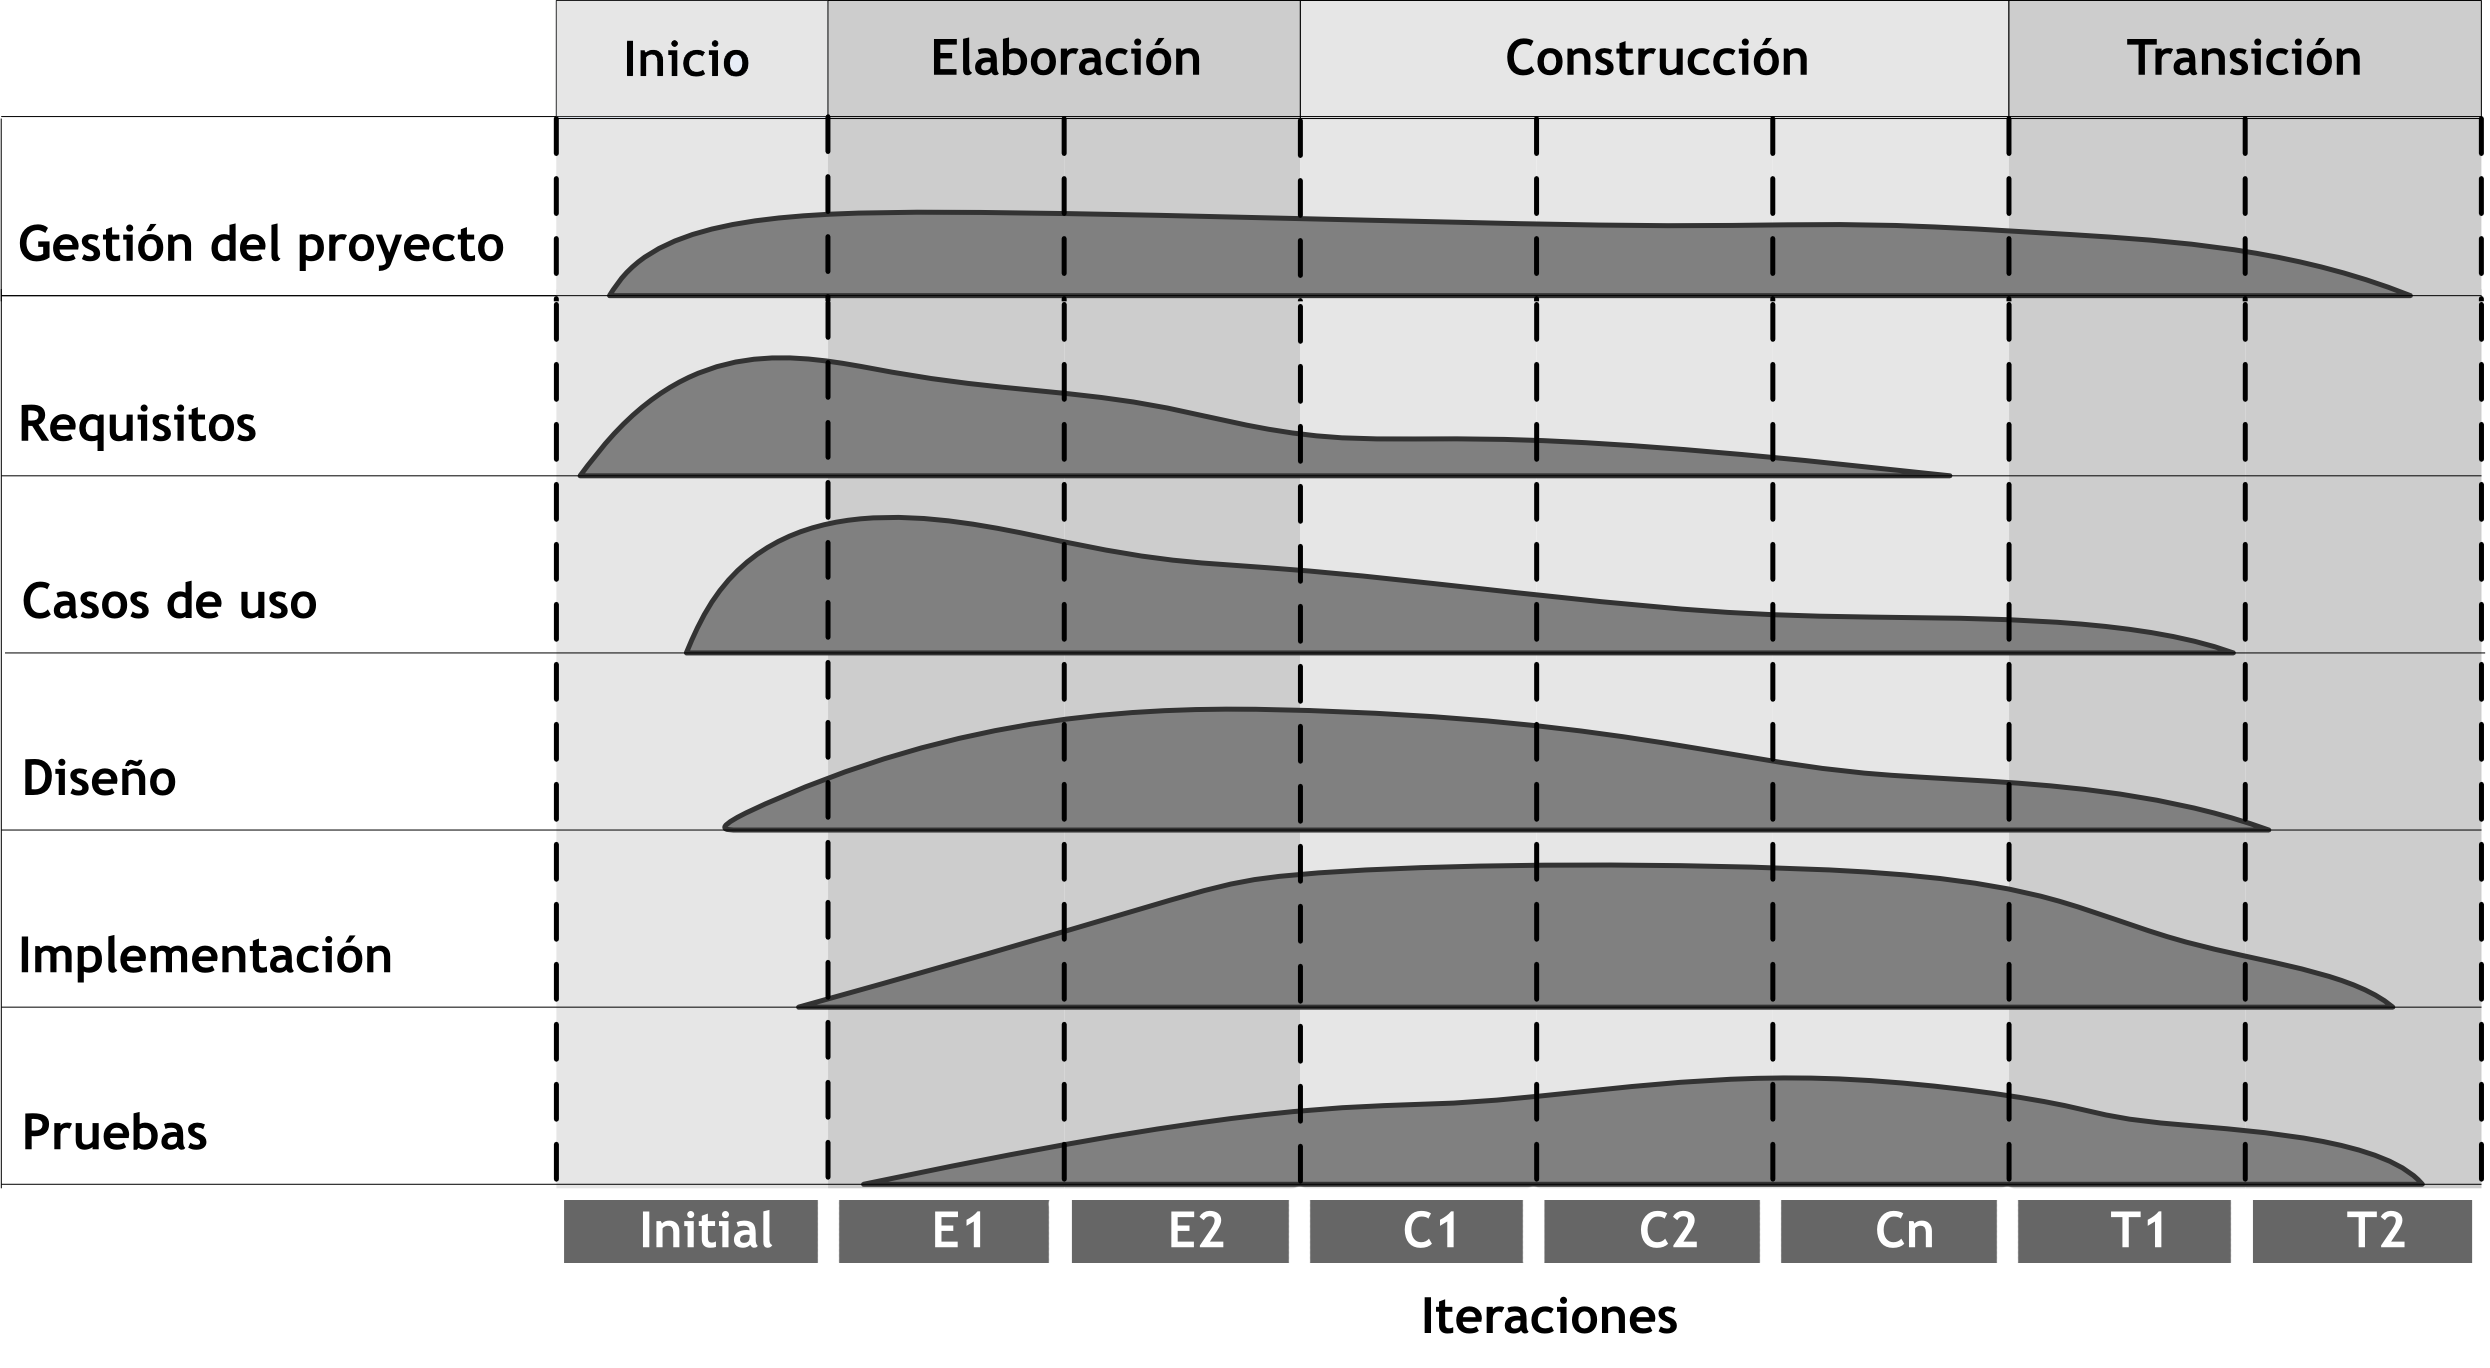
\includegraphics[width=\textwidth]{images/pud.png}
    \caption{Proceso Unificado de Desarrollo: etapas, entregables e iteraciones}
    \label{fig::pud}
  \end{center}
\end{figure}


\subsection{Visión global del proceso}

\acs{PUD} hace una clara distinción entre las dos dimensiones sobre las que se fundamenta el proceso, una dimensión estática y una dimensión dinámica:

\begin{itemize}
\item El eje horizontal representa el tiempo, y hace referencia al aspecto dinámico del proceso, en términos de \emph{etapas} e \emph{iteraciones}.
\item El eje vertical representa el aspecto estático del proceso, descrito en forma de \emph{actividades}, \emph{flujos de trabajo} o \emph{artefactos}\index{artefacto}.
\end{itemize}

En la figura \ref{fig::pud} se presenta gráficamente la estructuración del \acl{PUD} a lo largo de las dos dimensiones mencionadas.

\subsection{Etapas e iteraciones (dimensión dinámica)}

Tal y como se detalla en \cite{Rational1998}, el ciclo de vida del software según el \acl{PUD} se divide en 4 etapas o fases:

\begin{enumerate}
\item Fase de inicio
\item Fase de elaboración
\item Fase de construcción
\item Fase de transición
\end{enumerate}

La primera etapa, como inicio del desarrollo, tiene como finalidad el establecimiento de los requisitos del proyecto, los aspectos clave del mismo y las limitaciones conocidas para su desarrollo. En esta etapa se realiza la primera aproximación del modelo de casos de uso, y se presenta un plan de gestión del proyecto, detallando sus fases e iteraciones. Esta etapa puede concluir con la generación de un sencillo prototipo.

La fase de elaboración es la dedicada al análisis del dominio del problema, la aproximación de la arquitectura del sistema y la eliminación de los riesgos más críticos. Esta etapa es la más crítica, puesto que al finalizarla se puede considerar por terminada la \emph{ingeniería dura}. El diseño del sistema es el protagonista de esta fase. El análisis de requisitos y el modelo de casos de uso se dejan prácticamente terminados, y se da comienzo a la implementación.

La etapa de construcción es dedicada a desarrollar todos los componentes restantes y a integrarlos en el producto. Todas las características del software son probadas. Los esfuerzos se centran en la gestión de recursos y el control de operaciones para optimizar los costes, planificación y calidad. En esta etapa se crean los manuales de usuario.

El propósito de la fase de transición es la liberación del producto a la comunidad de usuarios. Una vez que el producto se entrega al usuario final, es posible que surjan problemas que corregir o se generen nuevos requisitos que deban ser implementados.

\subsection{Artefactos (dimensión estática)}

Un \emph{artefacto}\index{artefacto} es una pieza de información que es producida, modificada o utilizada por un proceso. Los artefactos son los productos tangibles del proyecto, los elementos generados durante el desarrollo hacia el producto final. Son la salida de una actividad y entrada de otra, y pueden ser modelos, documentos, archivos de código fuente, archivos ejecutables, etc.

Los artefactos generados durante el desarrollo de este proyecto, los cuales serán presentados más adelante, son los siguientes:

\begin{itemize}
\item Especificación de requisitos
\item Despliegue del sistema
\item Modelo de casos de uso
\item Diseño de la arquitectura software
\item Implementación
\item Documentación de pruebas
\end{itemize}



\section{Iteraciones}

En el apéndice \ref{chap::iteraciones} se ofrece un análisis detallado de la evolución iteracional del proceso de desarrollo del proyecto. En total se han realizado 7 iteraciones, cubriendo las etapas de Inicio, Elaboración y Construcción.

En el cuadro \ref{tabla::iteraciones} se ofrece un resumen de dichas estadísticas, mostrándose la evolución de cada artefacto con la conclusión de cada nueva iteración.


\begin{table}[h]  
  \begin{center}
    \begin{tabular}{|c|l||c||c|c||c|c|c|c|}
      \hline
      \tabheadformat
      -& -& Inicio & \multicolumn{2}{c||}{Elaboración} & \multicolumn{4}{c|}{Construcción}\\
      \hline
      \tabheadformat
      -& - & I1 & E1 & E2 & C1 & C2 & C3 & C4 \\
      \hline
      -& Duración & 75h & 50h & 50h & 75h & 125h & 80h & 70h \\
      \hline      \hline      
      \multirow{5}{*}{\begin{sideways}Artefactos\end{sideways}} & Requisitos & 53.6\% & 71.4\% & 85.7\% & 89.3\% & 96.4\% & 100\% & 100\% \\
      \cline{2-9}
      & Casos de uso & 27.8\% & 50\% & 77.8\% & 94.4\% & 100\% & 100\% & 100\%\\
      \cline{2-9}
      & Diseño & 10\% & 25\% & 75\% & 80\% & 85\% & 90\% & 95\% \\
      \cline{2-9}
      & Implementación & 0\% & 5.2\% & 17.3\% & 20.2\% & 50.8\% & 63.1\% & 75\% \\
      \cline{2-9}
      & Pruebas & 0\% & 0\% & 5\% & 10\% & 33.4\% & 59.1\% & 71\% \\
      \hline
    \end{tabular}
  \end{center}
  \caption{Evolución del proceso de desarrollo. Los porcentajes se han estimado teniendo en cuenta las líneas de código (para el caso de la implementación), la cobertura para las pruebas, y el número de elementos especificados (para el caso de los requisitos y los casos de uso)}
  \label{tabla::iteraciones}
\end{table}






\section{Análisis de requisitos}
\label{sec::requisitos}

Llegado este punto, procede estudiar los requisitos que debe satisfacer el sistema completo. En primer lugar se aproximará un listado de requisitos definidos de forma sencilla y superficial, para después realizar un análisis detallado de los mismos, siguiendo las directrices del estándar IEEE 830.

\subsection{Primera aproximación a los requisitos}

Para facilitar la visualización y posterior análisis de los mismos, se realiza la siguiente división:

\begin{itemize}
\item {\bf Requisitos de servidor}

  Requerimientos específicos del funcionamiento interno del sistema servidor, tanto del servidor web como del almacenamiento en base de datos y de comunicación.

\item {\bf Requisitos de usuario}

  Requerimientos asociados a la utilización por parte de un usuario. Están limitados a los aspectos referidos a los clientes del sistema.

\item {\bf Requisitos no funcionales}

  Requerimientos referidos a la seguridad, la evolución del software, al soporte, etc.


\end{itemize}

A continuación se enumeran los requisitos de cada grupo. Se trata de un análisis superficial. Con posterioridad se procederá a detallar esos requisitos.

\subsubsection{Funcionalidad referida al servidor}

La primera aproximación a los requisitos asociados al funcionamiento del sistema interno es la siguiente:

\begin{itemize}
\item El sistema debe permitir la comunicación con usuarios.
\item El sistema debe permitir almacenar y recuperar la información personal de los usuarios.
\item El sistema debe permitir almacenar y recuperar la evolución cerebral de los usuarios.
\item El sistema debe permitir recuperar listados de usuarios.
\item El sistema debe poder recomendar usuarios afines a uno dado.
\item El sistema debe poder recomendar juegos a los usuarios en base a su estado actual y evolución temporal.
\item El sistema debe ofrecer un listado con los juegos disponibles.
\item El sistema debe soportar la comunicación entre usuarios mediante mensajes escritos.
\end{itemize}


\subsubsection{Funcionalidad referida al usuario}


La primera aproximación a los requisitos asociados al usuario es la siguiente:

\begin{itemize}
\item Los usuarios podrán hacer uso de toda la web con cualquier navegador moderno, sin necesidad de plugins o componentes adicionales.
\item Los usuarios deben poder autenticarse en el sistema.
\item Los usuarios podrán cerrar su sesión.
\item Los usuarios no autenticados no deben tener acceso al resto del sitio web.
\item Los usuarios podrán registrarse.
\item El email de registro debe ser auténtico.
\item Los usuarios podrán recuperar su contraseña si no la recuerdan.
\item Los usuarios podrán seleccionar los parámetros cerebrales que deseen ejercitar.
\item Los usuarios podrán editar su información personal.
\item Los usuarios podrán seleccionar una imagen de avatar que les represente.
\item Los usuarios podrán seguir a otros usuarios.
\item Los usuarios podrán dejar de seguir a otros usuarios.
\item Los usuarios deben tener a su disposición un resumen de su evolución.
\item Los usuarios deben tener a su disposición un listado con noticias sobre los usuarios a los que sigue.
\item Los usuarios deben poder ver su perfil cerebral completo, con el estado actual y la evolución semanal, mensual y anual.
\item Los usuarios podrán hacer búsquedas de usuarios.
\item Los usuarios recibirán recomendaciones de juegos y de usuarios a los que seguir.
\item Los usuarios podrán visualizar un listado completo de juegos disponibles, diferenciando los juegos multijugador de los juegos de un solo jugador.
\item Los usuarios podrán ejecutar los juegos.
\end{itemize}

\subsubsection{Aspectos ajenos a la funcionalidad}

\begin{itemize}
\item El acceso a la base de datos debe ser rápido, para evitar esperas por parte del cliente.
\item La lógica de los juegos multijugador debe ser rápida, por lo que el servidor de juegos multijugador deberá tener muy buen rendimiento.
\item El rendimiento de los juegos deberá ser óptimo, por lo que el navegador de los clientes deberán ejecutar los juegos de forma eficiente.
\item El sistema debe soportar cientos de miles de peticiones simultáneas y responder de forma rápida y robusta.
\item El acceso al sistema debe ser controlado mediante email y contraseña.
\item Las personas no autenticadas no tendrán acceso a ninguna información ni juego.
\end{itemize}


\subsection{Requisitos funcionales}

Partiendo del análisis preliminar de requerimientos, los requisitos funcionales de los que parte el desarrollo del proyecto, basándose en el estándar IEEE 830, son los detallados a continuación. 

Para cada requisito se especifica una descripción sencilla del mismo, una valoración de su importancia (esencial, condicional u opcional), y una descripción de su validez, que incluye los mecanismos para medir su nivel de consecución, los medios para cumplir dicho requisito y una descripción de la relevancia que tiene dicho requisito en el desarrollo completo del sistema.

\renewcommand{\labelenumi}{\bf RF-\arabic{enumi}}

\begin{enumerate}

\item %%%%%%%%%%%%%%%%%%%%%%%%%%%%%%%%%%%%%%%%%%%%%%%%%%
  \begin{itemize}
  \item \underline{Descripción}: El sistema permitirá que los clientes se conecten al servidor e interactúen con la web.
  \item \underline{Importancia}: Esencial.
  \item \underline{Validez}:
    \begin{itemize}
    \item \textit{Medible}: El navegador web podrá conectarse al servidor web.
    \item \textit{Alcanzable}: El servidor ofrecerá una interfaz de peticiones GET y POST común.
    \item \textit{Relevante}: Este requisito es vital para la utilización del sistema por parte de los usuarios.
    \end{itemize}
  \end{itemize}

\item %%%%%%%%%%%%%%%%%%%%%%%%%%%%%%%%%%%%%%%%%%%%%%%%%%
  \begin{itemize}
  \item \underline{Descripción}: El sistema permitirá que los clientes intercambien mensajes con el servidor.
  \item \underline{Importancia}: Esencial.
  \item \underline{Validez}:
    \begin{itemize}
    \item \textit{Medible}: El navegador web y el servidor deben intercambiar mensajes.
    \item \textit{Alcanzable}: El servidor ofrecerá una interfaz de websockets para el intercambio de mensajes.
    \item \textit{Relevante}: Este requisito es vital para la utilización del sistema por parte de los usuarios.
    \end{itemize}
  \end{itemize}

\item %%%%%%%%%%%%%%%%%%%%%%%%%%%%%%%%%%%%%%%%%%%%%%%%%%
  \begin{itemize}
  \item \underline{Descripción}: El sistema permitirá almacenar y recuperar información personal de los usuarios.
  \item \underline{Importancia}: Esencial.
  \item \underline{Validez}:
    \begin{itemize}
    \item \textit{Medible}: El sistema recuperará la información personal de cualquier usuario dados su identificador y, por cuestiones de seguridad, su contraseña.
    \item \textit{Alcanzable}: El servidor estará conectado a una base de datos donde se almacenen y de donde se recuperen todos los datos.
    \item \textit{Relevante}: Este requisito es vital para que los usuarios puedan interactuar con el sistema.
    \end{itemize}
  \end{itemize}

\item %%%%%%%%%%%%%%%%%%%%%%%%%%%%%%%%%%%%%%%%%%%%%%%%%%
  \begin{itemize}
  \item \underline{Descripción}: El sistema permitirá almacenar y recuperar la evolución del entrenamiento cerebral de los usuarios.
  \item \underline{Importancia}: Esencial.
  \item \underline{Validez}:
    \begin{itemize}
    \item \textit{Medible}: El sistema recuperará el perfil cerebral de cualquier usuario dados su identificador y, por cuestiones de seguridad, su contraseña.
    \item \textit{Alcanzable}: El servidor estará conectado a una base de datos donde se almacenen y de donde se recuperen todos los datos.
    \item \textit{Relevante}: Este requisito es vital para que los usuarios puedan tener acceso a su evolución.
    \end{itemize}
  \end{itemize}

\item %%%%%%%%%%%%%%%%%%%%%%%%%%%%%%%%%%%%%%%%%%%%%%%%%%
  \begin{itemize}
  \item \underline{Descripción}: El sistema permitirá recuperar listados de usuarios.
  \item \underline{Importancia}: Esencial.
  \item \underline{Validez}:
    \begin{itemize}
    \item \textit{Medible}: El sistema realizará búsquedas en base a consultas textuales sencillas, obteniendo un listado con los resultados de la misma.
    \item \textit{Alcanzable}: El servidor estará conectado a una base de datos donde se almacenen todos los usuarios, y lanzará sobre ella consultas específicas.
    \item \textit{Relevante}: Este requisito es vital para que los usuarios puedan buscar a otros usuarios y empezar a seguirles, retarles a algún juego, etc.
    \end{itemize}
  \end{itemize}

\item %%%%%%%%%%%%%%%%%%%%%%%%%%%%%%%%%%%%%%%%%%%%%%%%%%
  \begin{itemize}
  \item \underline{Descripción}: El sistema recomendará juegos a los usuarios, en base a su evolución y características.
  \item \underline{Importancia}: Condicional
  \item \underline{Validez}:
    \begin{itemize}
    \item \textit{Medible}: Los usuarios tendrán en la sección de juegos un apartado con los juegos a los que el sistema les recomienda jugar, en base a su evolución cerebral.
    \item \textit{Alcanzable}: Se desarrollará un algoritmo de recomendación de juegos a usuarios basado en los parámetros cerebrales elegidos por ellos en su perfil y en la evolución de dichos parámetros a lo largo del tiempo.
    \item \textit{Relevante}: Este requisito es muy recomendable para mejorar la experiencia de usuario, además de para ayudar a mejorar las capacidades mentales en las que el usuario se vea menos hábil o cuya mejora le cueste más.
    \end{itemize}
  \end{itemize}

\item %%%%%%%%%%%%%%%%%%%%%%%%%%%%%%%%%%%%%%%%%%%%%%%%%%
  \begin{itemize}
  \item \underline{Descripción}: El sistema recomendará usuarios a los que seguir y retar, en base a sus preferencias y habilidades mentales.
  \item \underline{Importancia}: Condicional
  \item \underline{Validez}:
    \begin{itemize}
    \item \textit{Medible}: En la sección de búsqueda de usuarios de la web se ofrecerá un apartado con los usuarios más recomendables para el usuario actual.
    \item \textit{Alcanzable}: Se desarrollará un algoritmo de recomendación de personas a personas basado en los parámetros cerebrales elegidos por ellos en su perfil y en la evolución de dichos parámetros a lo largo del tiempo.
    \item \textit{Relevante}: Este requisito es muy recomendable para mejorar la experiencia de usuario, además de para ayudar a mejorar el aspecto social de BreakBrain.
    \end{itemize}
  \end{itemize}

\item %%%%%%%%%%%%%%%%%%%%%%%%%%%%%%%%%%%%%%%%%%%%%%%%%%
  \begin{itemize}
  \item \underline{Descripción}: El sistema ofrecerá un listado de juegos disponibles, permitiendo jugar a cualquiera de ellos.
  \item \underline{Importancia}: Esencial
  \item \underline{Validez}:
    \begin{itemize}
    \item \textit{Medible}: Los usuarios tendrán a su disposición un apartado de la web con todos los juegos disponibles.
    \item \textit{Alcanzable}: La web se dotará con una sección de juegos en la que se listen todos y cada uno de los juegos disponibles, categorizados por las capacidades mentales que ayudan a estimular.
    \item \textit{Relevante}: Este requisito es vital para conseguir que BreakBrain sea lo que se espera.
    \end{itemize}
  \end{itemize}

\item %%%%%%%%%%%%%%%%%%%%%%%%%%%%%%%%%%%%%%%%%%%%%%%%%%
  \begin{itemize}
  \item \underline{Descripción}: El sistema permitirá la comunicación entre usuarios mediante mensajes con el servidor.
  \item \underline{Importancia}: Esencial
  \item \underline{Validez}:
    \begin{itemize}
    \item \textit{Medible}: Los navegadores cliente de dos usuarios podrán comunicarse entre sí, de tal forma que puedan ejecutar juegos multijugador o comunicarse por medio de chat.
    \item \textit{Alcanzable}: Se emplearán websockets (un módulo en el cliente y otro en el servidor), para manterner una comunicación TCP full-duplex entre ambas partes. El servidor hará de intermediario entre dos clientes, simulando una comunicación directa entre ellos.
    \item \textit{Relevante}: Este requisito es vital para poder ofrecer juegos multijugador en la red social.
    \end{itemize}
  \end{itemize}

\item %%%%%%%%%%%%%%%%%%%%%%%%%%%%%%%%%%%%%%%%%%%%%%%%%%
  \begin{itemize}
  \item \underline{Descripción}: Los usuarios podrán hacer uso de la web completa ---incluyendo los juegos--- con cualquier navegador moderno, sin necesidad de plugins o extensiones adicionales.
  \item \underline{Importancia}: Condicional
  \item \underline{Validez}:
    \begin{itemize}
    \item \textit{Medible}: La web funcionará correctamente en diversos navegadores actuales, como las últimas versiones de Firefox, Chrome, Opera, etc.
    \item \textit{Alcanzable}: Se emplearán estándares web HTML5 y CSS3 para el desarrollo completo del sitio web, incluidos los juegos y cualquier otro componente de la red social.
    \item \textit{Relevante}: Se trata de un requisito importante, para imponer el mínimo número de restricciones al usuario final.
    \end{itemize}
  \end{itemize}


\item %%%%%%%%%%%%%%%%%%%%%%%%%%%%%%%%%%%%%%%%%%%%%%%%%%
  \begin{itemize}
  \item \underline{Descripción}: Los usuarios podrán autenticarse en el sistema para tener acceso a todo el sitio web.
  \item \underline{Importancia}: Esencial
  \item \underline{Validez}:
    \begin{itemize}
    \item \textit{Medible}: Al cargar BreakBrain se mostrará una pantalla de inicio de sesión, y ésta será la única visible hasta que el visitante inicie una sesión válida.
    \item \textit{Alcanzable}: El sitio web mantendrá un objeto de sesión con la información de usuario. Al iniciar sesión se creará dicho objeto, y al cerrarla se eliminará.
    \item \textit{Relevante}: Este es un requisito indispensable para que la web quede restringida a usuarios registrados y para que estos puedan consultar su evolución, seguir a otros usuarios, etc.
    \end{itemize}
  \end{itemize}

\item %%%%%%%%%%%%%%%%%%%%%%%%%%%%%%%%%%%%%%%%%%%%%%%%%%
  \begin{itemize}
  \item \underline{Descripción}: Los usuarios autenticados podrán cerrar su sesión.
  \item \underline{Importancia}: Condicional.
  \item \underline{Validez}:
    \begin{itemize}
    \item \textit{Medible}: En la parte superior derecha de la web (con una sesión iniciada) se mostrará un botón para cerrar sesión.
    \item \textit{Alcanzable}: El sitio web mantendrá un objeto de sesión con la información de usuario. Al iniciar sesión se creará dicho objeto, y al cerrarla se eliminará.
    \item \textit{Relevante}: Este requisito es importante para que diferentes usuarios puedan utilizar el mismo navegador.
    \end{itemize}
  \end{itemize}

\item %%%%%%%%%%%%%%%%%%%%%%%%%%%%%%%%%%%%%%%%%%%%%%%%%%
  \begin{itemize}
  \item \underline{Descripción}: Cualquier persona podrá registrarse para obtener una cuenta de usuario.
  \item \underline{Importancia}: Esencial
  \item \underline{Validez}:
    \begin{itemize}
    \item \textit{Medible}: Al acceder a BreakBrain sin una sesión iniciada, junto al formulario de login, aparecerá un formulario de registro para crear una cuenta de usuario.
    \item \textit{Alcanzable}: El sistema permitirá la creación de las estructuras de datos necesarias para la creación de un nuevo usuario, a petición de cualquier visitante desde la página de inicio.
    \item \textit{Relevante}: Es un requisito básico para que los usuarios puedan obtener una cuenta y utilizar la red social.
    \end{itemize}
  \end{itemize}

\item %%%%%%%%%%%%%%%%%%%%%%%%%%%%%%%%%%%%%%%%%%%%%%%%%%
  \begin{itemize}
  \item \underline{Descripción}: El email de registro debe ser auténtico.
  \item \underline{Importancia}: Condicional
  \item \underline{Validez}:
    \begin{itemize}
    \item \textit{Medible}: La red social no debe ser accesible a una cuenta de usuario hasta que el email haya sido correctamente comprobado.
    \item \textit{Alcanzable}: Durante el proceso de registro, el sistema debe asegurar que el email proporcionado es correcto. Para ello enviará a dicha dirección un enlace de activación. El usuario hará clic sobre el enlace para activar la cuenta y poder empezar a utilizarla.
    \item \textit{Relevante}: En BreakBrain, el identificador de los usuarios es su email. Por tanto, este requisito es importante para asegurar el contacto con cualquier usuario.
    \end{itemize}
  \end{itemize}

\item %%%%%%%%%%%%%%%%%%%%%%%%%%%%%%%%%%%%%%%%%%%%%%%%%%
  \begin{itemize}
  \item \underline{Descripción}: Los usuarios que no recuerden su contraseña podrán crear una nueva.
  \item \underline{Importancia}: Condicional
  \item \underline{Validez}:
    \begin{itemize}
    \item \textit{Medible}: La pantalla de inicio mostrará la posibilidad de solicitar un cambio de contraseña. Éste enviará un email al usuario, con un enlace de uno sólo uso que permita crear una nueva contraseña.
    \item \textit{Alcanzable}: Existirá una pantalla de establecimiento de contraseña, cuyo uso está restringido al acceso mediante enlaces generados por BreakBrain para los usuarios que lo soliciten. La base de datos mantendrá un hash por usuario, que será el utilizado para identificar un cambio de contraseña, generado cada vez que se utilice el anterior, para asegurar un único uso.
    \item \textit{Relevante}: Se trata de un requisito opcional, pero indispensable en caso de olvido de la contraseña.
    \end{itemize}
  \end{itemize}

\item %%%%%%%%%%%%%%%%%%%%%%%%%%%%%%%%%%%%%%%%%%%%%%%%%%
  \begin{itemize}
  \item \underline{Descripción}: Los usuarios podrán seleccionar qué parámetros cerebrales desean ejercitar y monitorizar.
  \item \underline{Importancia}: Condicional
  \item \underline{Validez}:
    \begin{itemize}
    \item \textit{Medible}: El perfil de usuario permitirá seleccionar las capacidades mentales que el usuario desee.
    \item \textit{Alcanzable}: La persistencia mantendrá un perfil cerebral con las capacidades mentales que deben ser consideradas por los algoritmos de recomendación y demás componentes del proyecto. Sólo los parámetros cerebrales que el usuario desee trabajar deberán ser tenidos en cuenta.
    \item \textit{Relevante}: Este requisito es importante para personalizar el entrenamiento cerebral. Si no se satisface, los usuarios no podrán priorizar las capacidades mentales.
    \end{itemize}
  \end{itemize}

\item %%%%%%%%%%%%%%%%%%%%%%%%%%%%%%%%%%%%%%%%%%%%%%%%%%
  \begin{itemize}
  \item \underline{Descripción}: Los usuarios podrán editar su información personal.
  \item \underline{Importancia}: Opcional
  \item \underline{Validez}:
    \begin{itemize}
    \item \textit{Medible}: El perfil le permitirá al usuario modificar su información personal.
    \item \textit{Alcanzable}: BreakBrain permitirá modificar todos los datos personales, menos el email, puesto que es el identificador de usuario y su autenticidad fue comprobada durante el proceso de registro.
    \item \textit{Relevante}: Es un requisito interesante para mejorar la experiencia de usuario.
    \end{itemize}
  \end{itemize}

\item %%%%%%%%%%%%%%%%%%%%%%%%%%%%%%%%%%%%%%%%%%%%%%%%%%
  \begin{itemize}
  \item \underline{Descripción}: Los usuarios podrán seleccionar una imagen de avatar para que les represente en la red.
  \item \underline{Importancia}: Opcional
  \item \underline{Validez}:
    \begin{itemize}
    \item \textit{Medible}: El perfil de usuario permitirá visualizar y modificar la imagen representativa del mismo.
    \item \textit{Alcanzable}: BreakBrain permitirá modificar los datos personales, incluida la imagen de avatar.
    \item \textit{Relevante}: Este requisito es poco importante, pero ayudará al usuario a mantener una imagen deseada frente al resto de usuarios, por lo que mejorará la experiencia de uso.
    \end{itemize}
  \end{itemize}

\item %%%%%%%%%%%%%%%%%%%%%%%%%%%%%%%%%%%%%%%%%%%%%%%%%%
  \begin{itemize}
  \item \underline{Descripción}: Los usuarios podrán comenzar a seguir a otros usuarios.
  \item \underline{Importancia}: Esencial
  \item \underline{Validez}:
    \begin{itemize}
    \item \textit{Medible}: La pantalla de exploración de usuarios permitirá comenzar a seguir a cualquier usuario.
    \item \textit{Alcanzable}: La persistencia mantendrá las estructuras de datos necesarias para almacenar qué usuarios siguen a qué otros usuarios.
    \item \textit{Relevante}: Este requisito es fundamental para mantener la componente social del proyecto.
    \end{itemize}
  \end{itemize}

\item %%%%%%%%%%%%%%%%%%%%%%%%%%%%%%%%%%%%%%%%%%%%%%%%%%
  \begin{itemize}
  \item \underline{Descripción}: Los usuarios podrán dejar de seguir a los usuarios a los que siguen.
  \item \underline{Importancia}: Esencial
  \item \underline{Validez}:
    \begin{itemize}
    \item \textit{Medible}: La pantalla de exploración de usuarios permitirá dejar de seguir a cualquier usuario.
    \item \textit{Alcanzable}: La persistencia mantendrá las estructuras de datos necesarias para almacenar qué usuarios siguen a qué otros usuarios.
    \item \textit{Relevante}: Este requisito es fundamental para mantener la componente social del proyecto.
    \end{itemize}
  \end{itemize}

\item %%%%%%%%%%%%%%%%%%%%%%%%%%%%%%%%%%%%%%%%%%%%%%%%%%
  \begin{itemize}
  \item \underline{Descripción}: Los usuarios podrán consultar un resumen de su evolución en la página de inicio.
  \item \underline{Importancia}: Condicional
  \item \underline{Validez}:
    \begin{itemize}
    \item \textit{Medible}: La pantalla principal mostrará un pequeño resumen de la evolución del perfil cerebral.
    \item \textit{Alcanzable}: El sistema deberá dar acceso a sólo parte del perfil cerebral y su evolución. La página principal mostrará, entre otras cosas, esa información resumida.
    \item \textit{Relevante}: La satisfacción de este requisito mejorará la experiencia de usuario, evitando que el mismo tenga que acceder al perfil completo para ver cómo va evolucionando.
    \end{itemize}
  \end{itemize}

\item %%%%%%%%%%%%%%%%%%%%%%%%%%%%%%%%%%%%%%%%%%%%%%%%%%
  \begin{itemize}
  \item \underline{Descripción}: Los usuarios podrán consultar un listado de novedades sobre los usuarios a los que siguen en la página de inicio.
  \item \underline{Importancia}: Condicional
  \item \underline{Validez}:
    \begin{itemize}
    \item \textit{Medible}: La página principal del sitio web mostrará las novedades de los usuarios a los que se sigue.
    \item \textit{Alcanzable}: El perfil de cada usuario incluirá un pequeño listado de novedades. Los usuarios que sigan a uno dado, y sólo ellos, tendrán acceso a dicho listado.
    \item \textit{Relevante}: La satisfacción de este requisito mejorará la experiencia de usuario, sobre todo en el aspecto social.
    \end{itemize}
  \end{itemize}

\item %%%%%%%%%%%%%%%%%%%%%%%%%%%%%%%%%%%%%%%%%%%%%%%%%%
  \begin{itemize}
  \item \underline{Descripción}: Los usuarios podrán ver su perfil cerebral completo, con el estado actual y la evolución semanal, mensual y anual.
  \item \underline{Importancia}: Esencial
  \item \underline{Validez}:
    \begin{itemize}
    \item \textit{Medible}: La web contará con una página dedicada al perfil y evolución cerebral.
    \item \textit{Alcanzable}: El sistema manejará una estructura de datos compleja con toda la información relevante referida al cerebro. Esta información incluirá el estado actual y la evolución del mismo a lo largo del tiempo.
    \item \textit{Relevante}: Se trata de un requisito vital para alcanzar los objetivos del proyecto.
    \end{itemize}
  \end{itemize}

\item %%%%%%%%%%%%%%%%%%%%%%%%%%%%%%%%%%%%%%%%%%%%%%%%%%
  \begin{itemize}
  \item \underline{Descripción}: Los usuarios podrán hacer búsquedas de usuarios.
  \item \underline{Importancia}: Esencial
  \item \underline{Validez}:
    \begin{itemize}
    \item \textit{Medible}: Existirá una página de exploración de usuarios que permitirá realizar búsquedas filtradas sobre todo el directorio de usuarios.
    \item \textit{Alcanzable}: Se desarrollará un algoritmo de búsqueda de usuarios, y será puesto a disposición de todos los usuarios mediante un sencillo formulario de búsqueda.
    \item \textit{Relevante}: Este requisito es de obligado cumplimiento para mantener un aspecto social completo en el proyecto, permitiendo que los usuarios puedan encontrar a otros usuarios y comenzar a seguirlos, dejar de seguirlos, retarles a juegos multijugador, etc.
    \end{itemize}
  \end{itemize}

\item %%%%%%%%%%%%%%%%%%%%%%%%%%%%%%%%%%%%%%%%%%%%%%%%%%
  \begin{itemize}
  \item \underline{Descripción}: Los usuarios recibirán recomendaciones de juegos.
  \item \underline{Importancia}: Condicional
  \item \underline{Validez}:
    \begin{itemize}
    \item \textit{Medible}: La web mostrará un apartado con juegos recomendados para el usuario actual.
    \item \textit{Alcanzable}: Se desarrollará un algoritmo de recomendación de juegos completo, basado en la evolución cerebral de los usuarios y su afinidad a cada tipo de juegos.
    \item \textit{Relevante}: Se trata de un requerimiento importante para mejorar la experiencia de usuario y asegurar una mejora cerebral equilibrada, reforzando las capacidades en los que el usuario flaquee más.
    \end{itemize}
  \end{itemize}

\item %%%%%%%%%%%%%%%%%%%%%%%%%%%%%%%%%%%%%%%%%%%%%%%%%%
  \begin{itemize}
  \item \underline{Descripción}: Los usuarios recibirán recomendaciones de usuarios a los que seguir.
  \item \underline{Importancia}: Condicional.
  \item \underline{Validez}:
    \begin{itemize}
    \item \textit{Medible}: La web mostrará un apartado con usuarios recomendados para el usuario actual.
    \item \textit{Alcanzable}: Se desarrollará un algoritmo de recomendación de juegos completo, basado en la evolución cerebral de los usuarios y su afinidad a cada tipo de juegos.
    \item \textit{Relevante}: Es un requisito importante para mejorar la experiencia de usuario.
    \end{itemize}
  \end{itemize}

\item %%%%%%%%%%%%%%%%%%%%%%%%%%%%%%%%%%%%%%%%%%%%%%%%%%
  \begin{itemize}
  \item \underline{Descripción}: Los usuarios podrán visualizar un listado completo de juegos disponibles, diferenciando los juegos multijugador de los juegos de un sólo jugador.
  \item \underline{Importancia}: Esencial
  \item \underline{Validez}:
    \begin{itemize}
    \item \textit{Medible}: La web ofrecerá un listado con todos los juegos disponibles, permitiendo que el usuario ejecute el que desee.
    \item \textit{Alcanzable}: El sistema mantendrá un catálogo categorizado con todos los juegos disponibles.
    \item \textit{Relevante}: Este requisito es vital para satisfacer los objetivos de BreakBrain.
    \end{itemize}
  \end{itemize}

\item %%%%%%%%%%%%%%%%%%%%%%%%%%%%%%%%%%%%%%%%%%%%%%%%%%
  \begin{itemize}
  \item \underline{Descripción}: Los usuarios podrán retar a otros usuarios y ser retados para jugar a juegos multijugador.
  \item \underline{Importancia}: Condicional
  \item \underline{Validez}:
    \begin{itemize}
    \item \textit{Medible}: La web ofrecerá un listado con todos los juegos disponibles, permitiendo que el usuario ejecute el que desee. En caso de ser un juego multijugador permitirá elegir a otro usuario contra el que jugar.
    \item \textit{Alcanzable}: El sistema permitirá seleccionar un usuario rival para jugar a un juego multijugador. Se enviará un mensaje de alerta al mismo para avisarle del reto y permitirle aceptarlo o rechazarlo.
    \item \textit{Relevante}: Este requisito es importante para satisfacer el objetivo social de BreakBrain.
    \end{itemize}
  \end{itemize}


\end{enumerate}

\subsection{Requisitos de evolución}

Partiendo del análisis preliminar de requerimientos, los requisitos de evolución de los que parte el desarrollo del proyecto, basándose en el estándar IEEE 830, son los siguientes:

\renewcommand{\labelenumi}{\bf EV-\arabic{enumi}}

\begin{enumerate}

\item %%%%%%%%%%%%%%%%%%%%%%%%%%%%%%%%%%%%%%%%%%%%%%%%%%
  \begin{itemize}
  \item \underline{Descripción}: El sistema debe soportar la integración de juegos desarrollados por terceros.
  \item \underline{Importancia}: Condicional
  \item \underline{Validez}:
    \begin{itemize}
    \item \textit{Medible}: Cualquier persona podrá crear juegos para la red social.
    \item \textit{Alcanzable}: Existirá un cargador de juegos genérico, así como un pequeño framework de construcción de los mismos, para posibilitar la compatibilidad con el sistema de comunicación cliente-servidor del sistema.
    \item \textit{Relevante}: Es un requisito interesante para facilitar la expansión de la red social, permitiendo tener contenidos nuevos de forma frecuente.
    \end{itemize}
  \end{itemize}

\end{enumerate}

\subsection{Requisitos de soporte}

Partiendo del análisis preliminar de requerimientos, los requisitos de soporte de los que parte el desarrollo del proyecto, basándose en el estándar IEEE 830, son los siguientes:
\renewcommand{\labelenumi}{\bf SO-\arabic{enumi}}

\begin{enumerate}

\item %%%%%%%%%%%%%%%%%%%%%%%%%%%%%%%%%%%%%%%%%%%%%%%%%%
  \begin{itemize}
  \item \underline{Descripción}: El acceso a la web debe realizarse desde un navegador moderno.
  \item \underline{Importancia}: Esencial
  \item \underline{Validez}:
    \begin{itemize}
    \item \textit{Medible}: El rendimiento en navegadores obsoletos dejará mucho que desear, siendo estos incluso incompatibles con ciertos componentes de la última especificación del estándar HTML5, como el canvas.
    \item \textit{Alcanzable}: Se utilizarán elementos compatibles con Firefox 9+, Chrome/Chromium 15+, Safari 5+ y Opera 12+.
    \item \textit{Relevante}: Este requisito es de vital cumplimiento para que la experiencia de usuario sea satisfactoria.
    \end{itemize}
  \end{itemize}

\end{enumerate}

\subsection{Requisitos de calidad}

Partiendo del análisis preliminar de requerimientos, los requisitos de soporte de los que parte el desarrollo del proyecto, basándose en el estándar IEEE 830, son los siguientes:
\renewcommand{\labelenumi}{\bf CA-\arabic{enumi}}

\begin{enumerate}

\item %%%%%%%%%%%%%%%%%%%%%%%%%%%%%%%%%%%%%%%%%%%%%%%%%%
  \begin{itemize}
  \item \underline{Descripción}: Los usuarios no autenticados no podrán acceder al contenido del sitio web.
  \item \underline{Importancia}: Esencial
  \item \underline{Validez}:
    \begin{itemize}
    \item \textit{Medible}: Cuando un visitante no autenticado acceda a cualquier página de la web, éste será redireccionado a la página de inicio (login).
    \item \textit{Alcanzable}: La descarga de cualquier contenido de la web será posible únicamente desde una cuenta de usuario válida, por lo que ningún visitante no autenticado tendrá acceso a ninguna información.
    \item \textit{Relevante}: Este requisito es importante para mantener la privacidad dentro de la red social.
    \end{itemize}
  \end{itemize}

\item %%%%%%%%%%%%%%%%%%%%%%%%%%%%%%%%%%%%%%%%%%%%%%%%%%
  \begin{itemize}
  \item \underline{Descripción}: La base de datos almacenará la información de los usuarios de forma segura.
  \item \underline{Importancia}: Esencial
  \item \underline{Validez}:
    \begin{itemize}
    \item \textit{Medible}: Toda la información vital de los usuarios será almacenada de forma encriptada.
    \item \textit{Alcanzable}: Los datos sensibles de los usuarios se almacenarán de forma encriptada.
    \item \textit{Relevante}: Requisito importante para mantener la seguridad en el almacenamiento de la información.
    \end{itemize}
  \end{itemize}

\item %%%%%%%%%%%%%%%%%%%%%%%%%%%%%%%%%%%%%%%%%%%%%%%%%%
  \begin{itemize}
  \item \underline{Descripción}: La comunicación entre el cliente y el servidor será segura.
  \item \underline{Importancia}: Esencial
  \item \underline{Validez}:
    \begin{itemize}
    \item \textit{Medible}: Toda la información vital de los usuarios será enviada al servidor de forma encriptada.
    \item \textit{Alcanzable}: Los datos sensibles de los usuarios se encriptarán localmente antes de ser enviados al servidor.
    \item \textit{Relevante}: Requisito muy importante para garantizar la seguridad de la transmisión de información.
    \end{itemize}
  \end{itemize}


\item %%%%%%%%%%%%%%%%%%%%%%%%%%%%%%%%%%%%%%%%%%%%%%%%%%
  \begin{itemize}
  \item \underline{Descripción}: La información de sesión local se almacenará de forma segura.
  \item \underline{Importancia}: Esencial
  \item \underline{Validez}:
    \begin{itemize}
    \item \textit{Medible}: La información sensible que se permanezca guardada localmente será ilegible.
    \item \textit{Alcanzable}: Los datos sensibles serán encriptados antes de almacenarse de forma local.
    \item \textit{Relevante}: Requisito importante para mantener la seguridad del software.
    \end{itemize}
  \end{itemize}

\item %%%%%%%%%%%%%%%%%%%%%%%%%%%%%%%%%%%%%%%%%%%%%%%%%%
  \begin{itemize}
  \item \underline{Descripción}: El servidor debe ofrecer tiempos de respuesta muy bajos, para evitar retardos en el uso de la web o los juegos.
  \item \underline{Importancia}: Esencial
  \item \underline{Validez}:
    \begin{itemize}
    \item \textit{Medible}: La utilización de la web debe ser fluida.
    \item \textit{Alcanzable}: Se desarrollará un servidor con buen rendimiento y tiempos de respuesta bajos. Se utilizará MongoDB como base de datos, para asegurar un rendimiento óptimo en la recuperación de información.
    \item \textit{Relevante}: Cumplir este requisito será esencial para que la experiencia de usuario sea buena.
    \end{itemize}
  \end{itemize}

\item %%%%%%%%%%%%%%%%%%%%%%%%%%%%%%%%%%%%%%%%%%%%%%%%%%
  \begin{itemize}
  \item \underline{Descripción}: Los juegos deben ofrecer una interacción sencilla.
  \item \underline{Importancia}: Condicional
  \item \underline{Validez}:
    \begin{itemize}
    \item \textit{Medible}: Cualquier persona no debería tener dificultad para jugar a los juegos de la plataforma.
    \item \textit{Alcanzable}: Los controles de los juegos serán preferiblemente mediante el uso del ratón o de un número bajo de teclas. Serán intuitivos, como el uso de las flechas del teclado.
    \item \textit{Relevante}: Requisito altamente recomendable para asegurar una buena  jugabilidad.
    \end{itemize}
  \end{itemize}

\item %%%%%%%%%%%%%%%%%%%%%%%%%%%%%%%%%%%%%%%%%%%%%%%%%%
  \begin{itemize}
  \item \underline{Descripción}: El sistema debe ser escalable, es decir, debe permitir aumentar la capacidad de trabajo sin comprometer su funcionamiento y calidad normales. 
  \item \underline{Importancia}: Esencial
  \item \underline{Validez}:
    \begin{itemize}
    \item \textit{Medible}: Podrá conectarse un gran número de usuarios de forma simultánea y realizar varias peticiones de información, juegos, etc. sin que el sistema sufra pérdida de rendimiento.
    \item \textit{Alcanzable}: Se empleará NodeJS\index{nodejs} para la construcción del servidor, así como MongoDB para la persistencia.
    \item \textit{Relevante}: Este requisito es vital para el proyecto en construcción, dado que una red social puede sufrir un gran número de conexiones simultáneas.
    \end{itemize}
  \end{itemize}

\end{enumerate}



\section{Diagrama de despliegue}
\label{sec::despliegue}

En base a la caracterización del sistema producida por el análisis de requisitos desarrollado a lo largo de la sección \ref{sec::requisitos} se ha elaborado el diagrama de despliegue de la figura \ref{fig::despliegue}. Nótese que se trata de una arquitectura cliente-servidor típica.

\begin{figure}[h]
  \begin{center}
    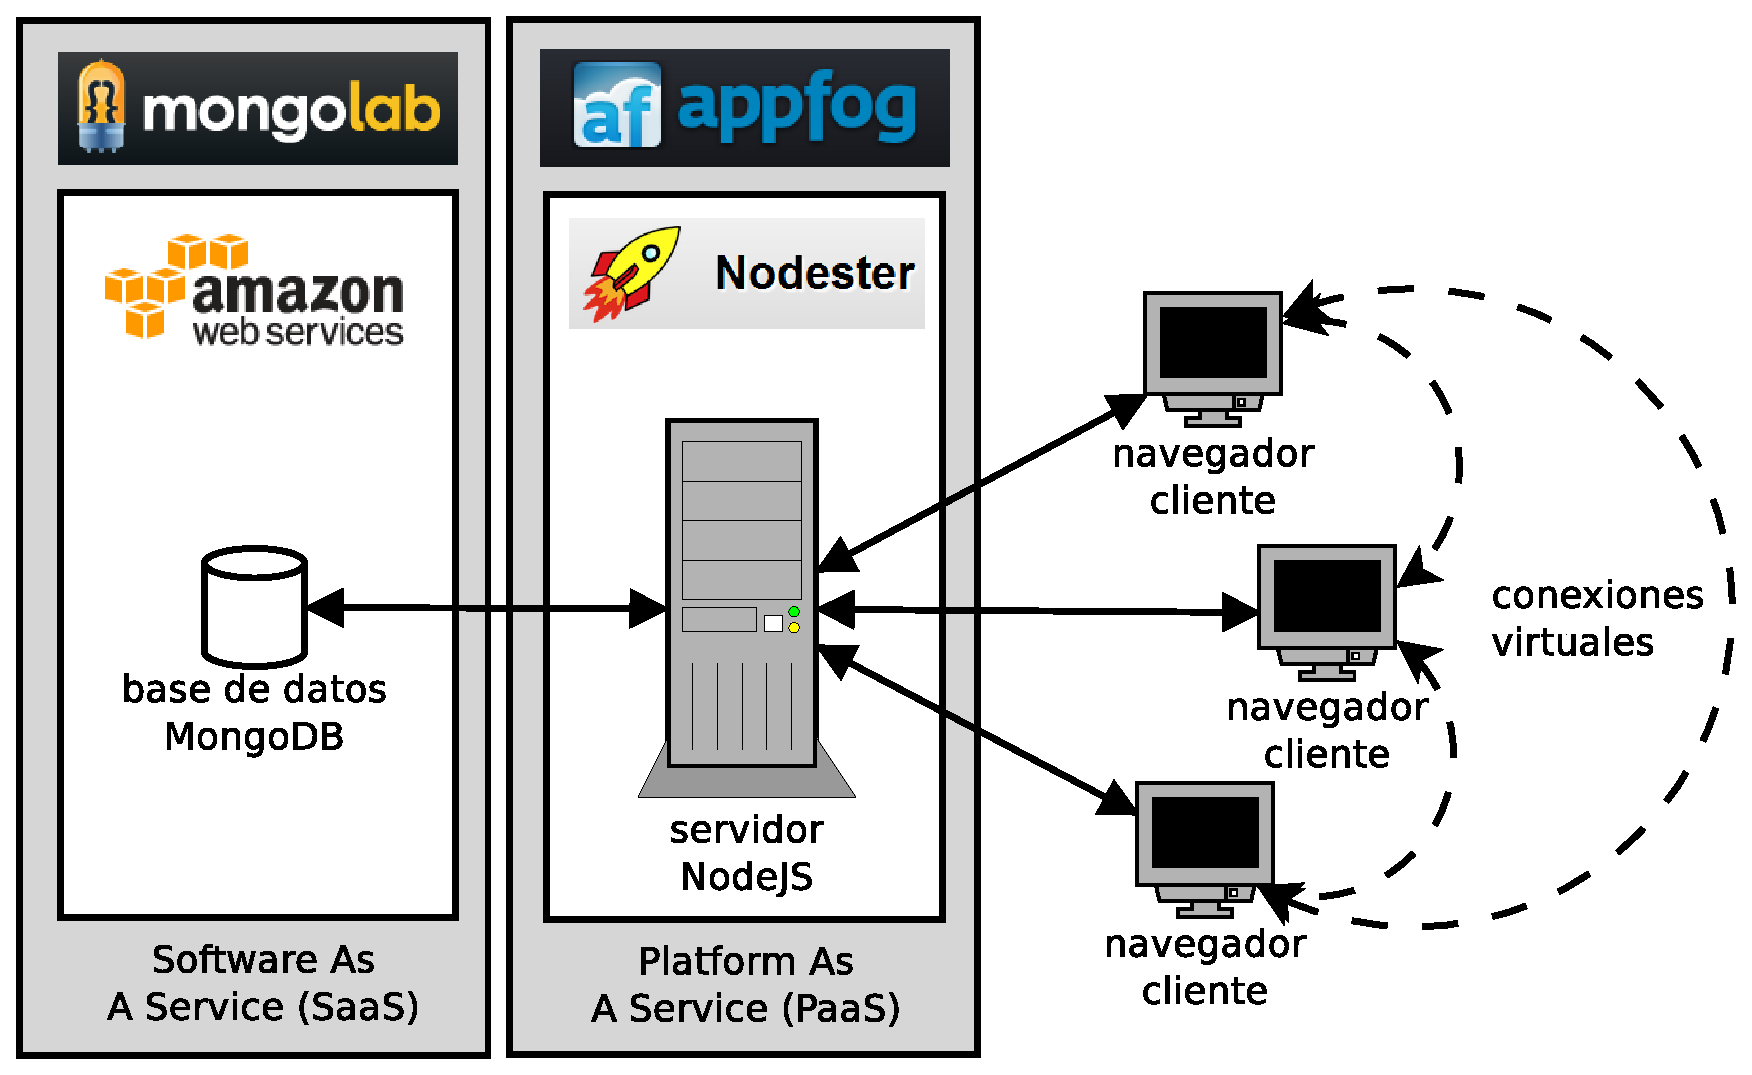
\includegraphics[width=\textwidth]{images/despliegue.eps}
    \caption{Diagrama de despliegue del sistema completo}
    \label{fig::despliegue}
  \end{center}
\end{figure}

Como puede apreciarse en la figura \ref{fig::despliegue} se emplean servicios externos que satisfacen las necesidades del sistema:

\begin{itemize}
\item Por un lado se hace uso del servicio {\bf MongoLab} \cite{Mongolab}, que proporciona un \ac{SGBD} funcionando como lo que se conoce como \ac{SAAS}, con MongoDB \cite{MongoDB}\index{mongodb} como base de datos. La persistencia de la base de datos tiene lugar en los servicios de almacenamiento web de Amazon \cite{Amazon}.
\item Por otro lado, el servidor del sistema es alojado en {\bf Nodester} \cite{Nodester}, una plataforma/hosting de aplicaciones web construidas con NodeJS \cite{NodeJS}\index{nodejs}. Este servicio pertenece a lo que se conoce como \ac{PAAS}, y es ofrecido por AppFog \cite{AppFog}.
\end{itemize}


\section{Análisis de casos de uso}
\label{sec::casos}

En esta sección se detalla el proceso seguido para la generación del artefacto correspondiente al análisis de casos de uso del sistema. En primer lugar se realiza una identificación de los actores que intervienen, para después dar paso a la identificación de los casos de uso. Por último éstos son especificados mediante una descripción, el listado de requisitos asociados, los actores que intervienen, las precondiciones y postcondiciones, los flujos de eventos y los posibles casos de uso asociados.

\subsection{Identificación  de actores}

Considerando el sistema en construcción como un único bloque, los actores que interactúan con él son los visitantes (no autenticados), los usuarios del mismo (personas autenticadas) y el sistema gestor de base de datos, al tratarse de un servicio externo. Así pues, los actores que interacturarán con los casos de uso son los siguientes:

\begin{itemize}
\item Visitante
\item Usuario
\item Sistema Gestor de Base de Datos (SGBD)
\end{itemize}

\subsection{Identificación de casos de uso}

En base al estudio de requisitos realizado en la sección \ref{sec::requisitos}, los casos de uso que se han identificado y pasarán a ser detallados como base de las etapas posteriores del desarrollo son los mostrados en la figura \ref{fig::casos}.

\begin{figure}[H]
  \begin{center}
    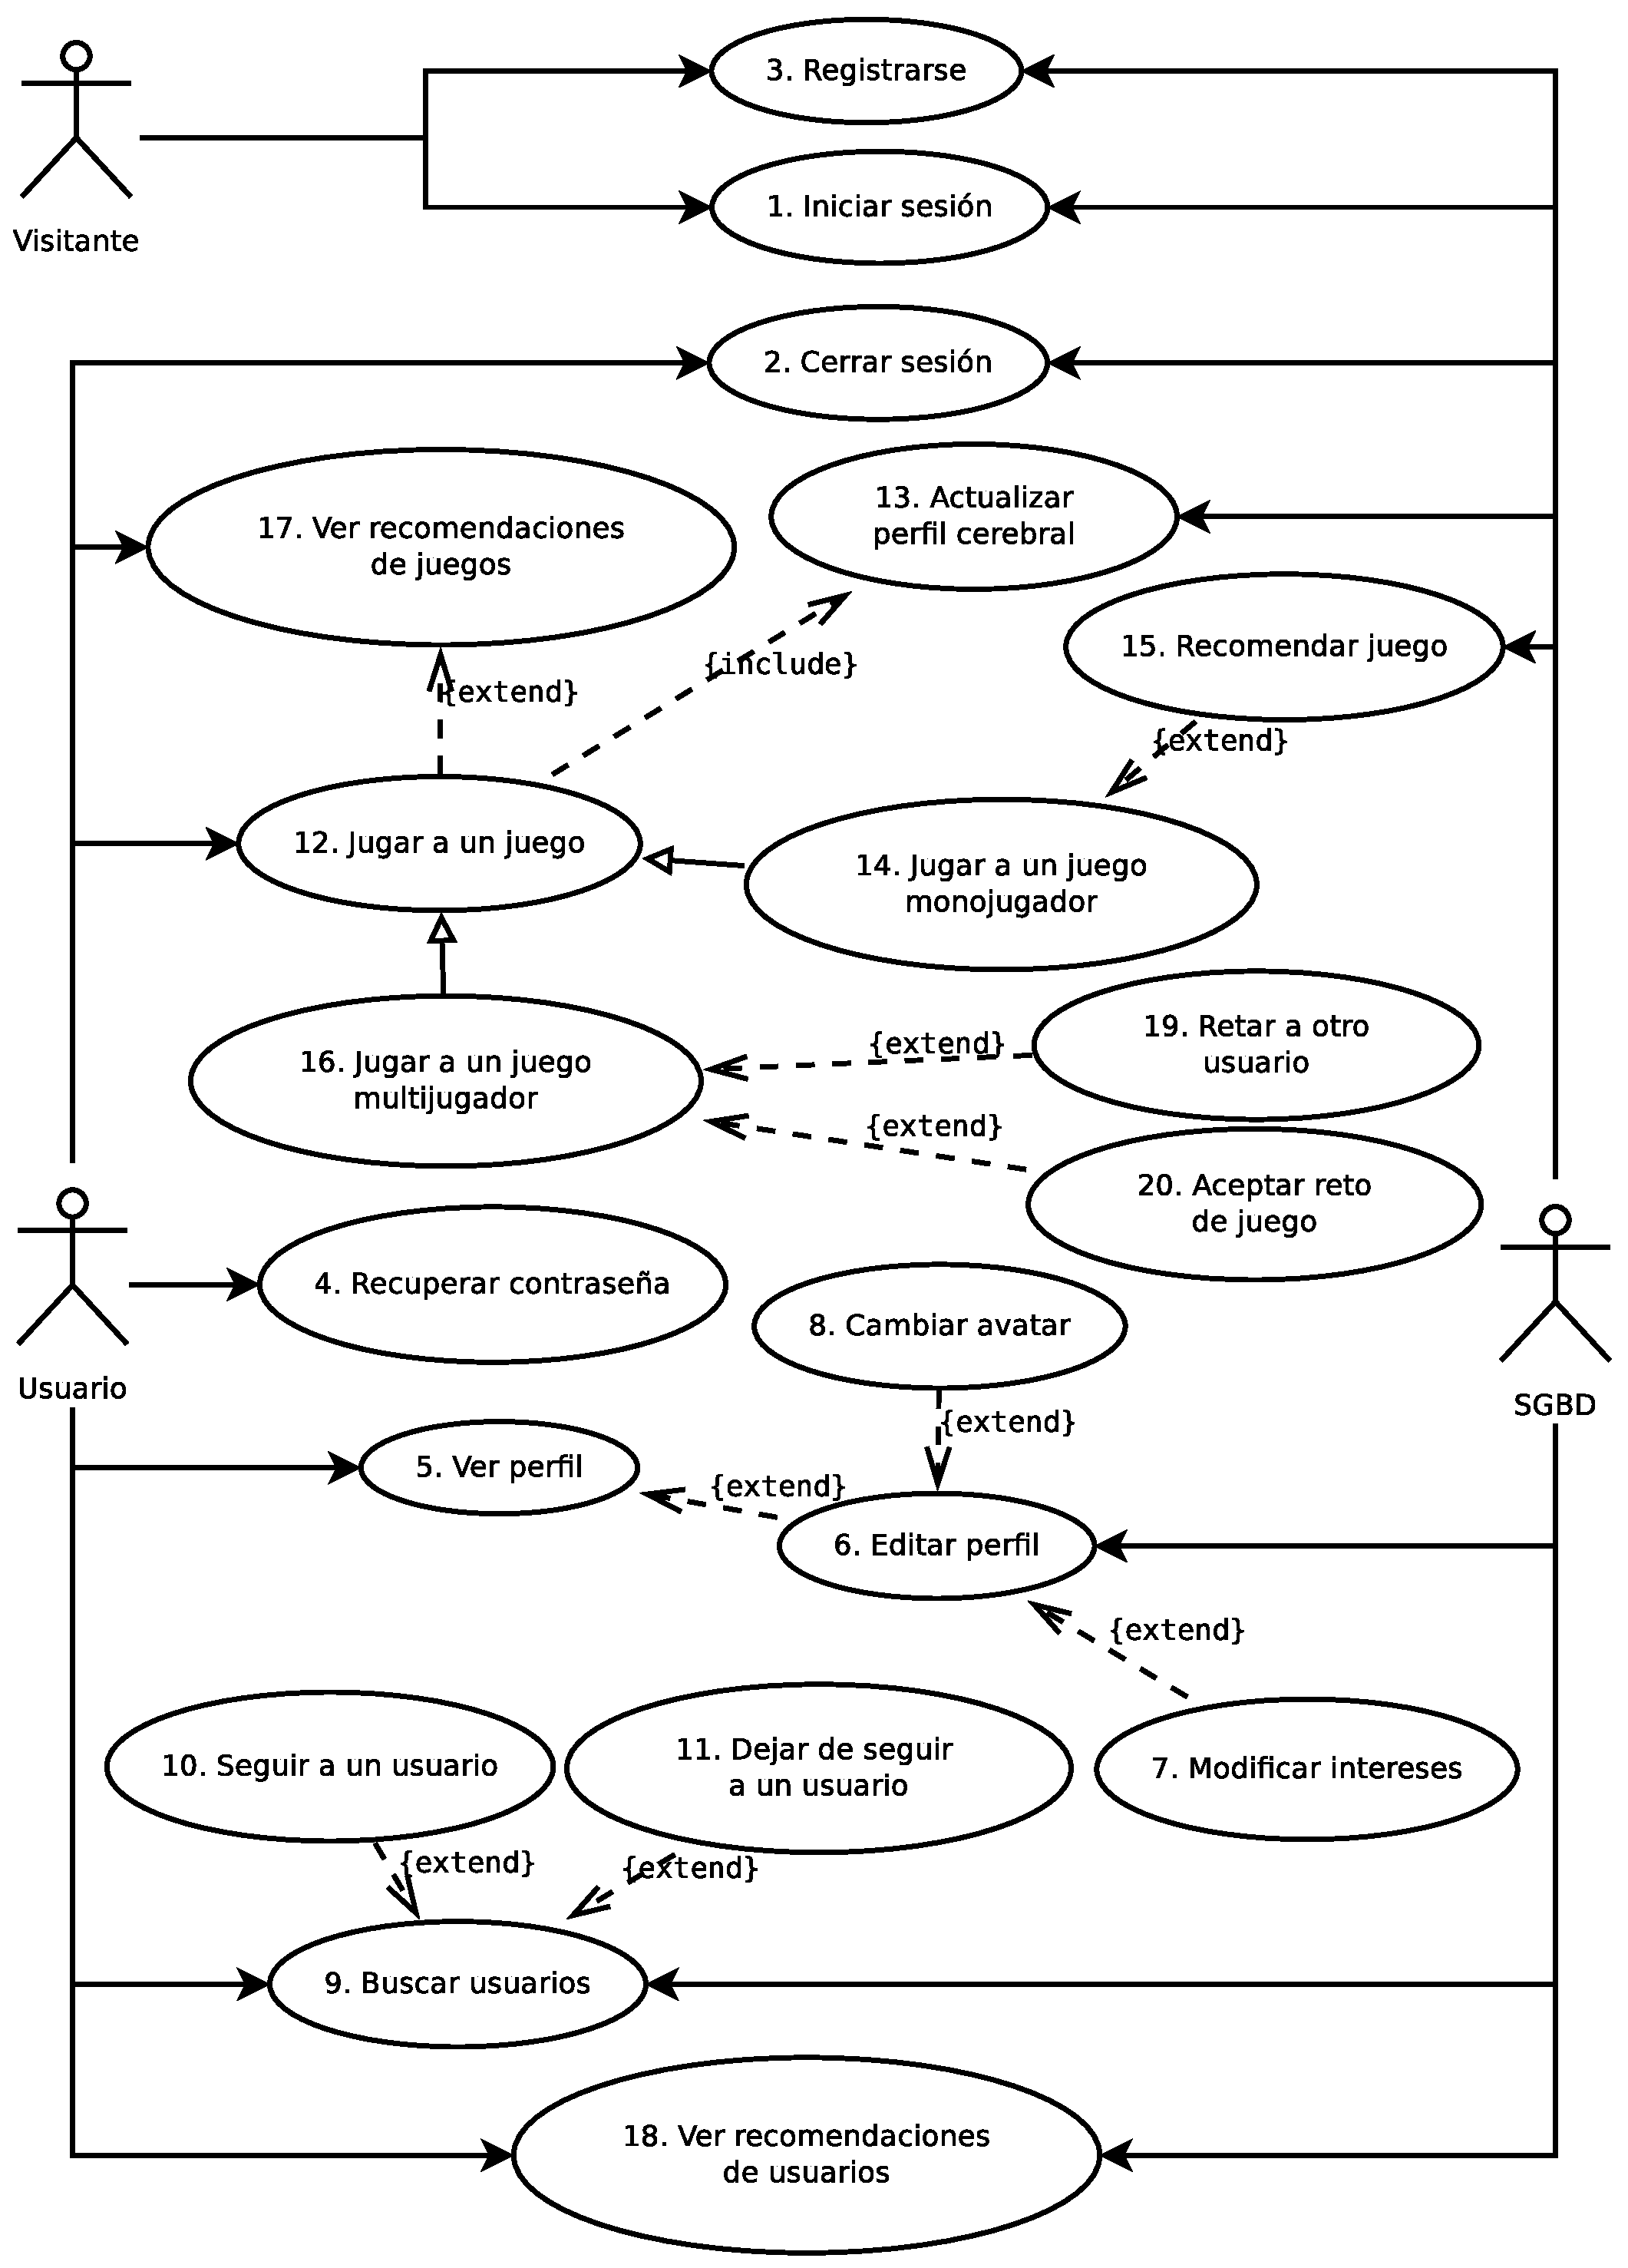
\includegraphics[width=0.9\textwidth]{images/casos-uso.eps}
    \caption{Diagrama de casos de uso}
    \label{fig::casos}
  \end{center}
\end{figure}


\subsection{Especificación de casos de uso}

A continuación se detallan todos los casos de uso identificados en la etapa anterior. Los más identificativos se acompañan, además, de un diagrama de secuencia para facilitar la comprensión del funcionamiento interno del sistema.

\renewcommand{\labelenumi}{\bf UC-\arabic{enumi}}
\renewcommand{\labelenumii}{\arabic{enumii}. }

\begin{enumerate}
\itemsep1cm
\item %%%%%%%%%%%%%%%%%%%%%%%%%%%%%%%%%%%%%%%%%%%%%%%%%%
  \begin{itemize}
  \item \textbf{Caso de uso}: Iniciar sesión
  \item \textbf{Requisito funcional asociado}: RF-11
  \item \textbf{Actores}
    \begin{itemize}
    \item Visitante
    \item SGBD
    \end{itemize}
  \item \textbf{Descripción}: Un visitante de la web inicia sesión.
  \item \textbf{Precondiciones}
    \begin{itemize}
    \item La persona no está autenticada.
    \end{itemize}
  \item \textbf{Postcondiciones}
    \begin{itemize}
    \item La persona queda autenticada (es un usuario de la red social), y tiene acceso al contenido de la web.
    \end{itemize}
  \item \textbf{Flujo normal}: autenticación exitosa (figura \ref{fig::uc-1})
    \begin{enumerate}
    \item El usuario rellena el formulario de login (email + contraseña) de la web.
    \item La web realiza la petición de envío al módulo cliente de websockets.
    \item El módulo cliente de websockets envía la petición al módulo servidor de websockets.
    \item El módulo servidor de websockets analiza la petición y se la pasa a la lógica del servidor.
    \item El módulo de lógica de servidor transforma la petición y solicita al módulo de persistencia la comprobación de los datos.
    \item El módulo de persistencia solicita al SGBD el usuario asociado al par email/contraseña.
    \item El SGBD devuelve el objeto que representa al usuario al módulo de persistencia.
    \item El módulo de persistencia transforma el objeto de usuario a la representación de dominio de un usuario y devuelve el resultado a la lógica del sistema.
    \item La lógica comprueba que el usuario es correcto y solicita su envío hacia el cliente al módulo servidor de websockets.
    \item El módulo servidor de websockets envía el objeto de usuario al módulo cliente de websockets.
    \item El módulo cliente de websockets pasa el objeto a la web.
    \item La web se actualiza con la información básica del usuario y muestra el contenido interno de la red social.
    \end{enumerate}
  \item \textbf{Flujo alternativo 1}: contraseña incorrecta o usuario inexistente
    \begin{enumerate}
    \item El usuario rellena el formulario de login (email + contraseña) de la web.
    \item La web realiza la petición de envío al módulo cliente de websockets.
    \item El módulo cliente de websockets envía la petición al módulo servidor de websockets.
    \item El módulo servidor de websockets analiza la petición y se la pasa a la lógica del servidor.
    \item El módulo de lógica de servidor transforma la petición y solicita al módulo de persistencia la comprobación de los datos.
    \item El módulo de persistencia solicita al SGBD el usuario asociado al par email/contraseña.
    \item El SGBD devuelve un error de correspondencia email/contraseña o de contraseña incorrecta.
    \item El módulo de persistencia transforma el error a la representación de dominio y lo devuelve al módulo de lógica del sistema.
    \item La lógica solicita el envío del error hacia el cliente al módulo servidor de websockets.
    \item El módulo servidor de websockets envía el error al módulo cliente de websockets.
    \item El módulo cliente de websockets pasa el error a la web.
    \item La web muestra un error de ``contraseña incorrecta'' o ``usuario inexistente'', según proceda.
    \end{enumerate}
  \item \textbf{Includes}
    \begin{itemize}
    \item Ninguno
    \end{itemize}
  \item \textbf{Extensiones}
    \begin{itemize}
    \item Ninguna
    \end{itemize}
  \item {\bf Diagrama de interacción}: Figura \ref{fig::uc-1}
  \end{itemize}


  \begin{figure}[h]
    \begin{center}
      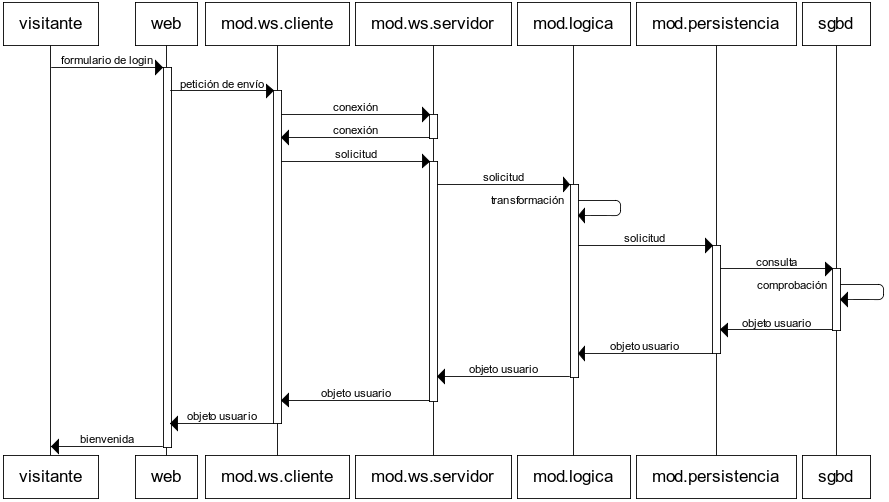
\includegraphics[width=\textwidth]{images/uc-1.png}
      \caption{Diagrama de interacción del caso de uso UC-1 (flujo normal)}
      \label{fig::uc-1}
    \end{center}
  \end{figure}


\item %%%%%%%%%%%%%%%%%%%%%%%%%%%%%%%%%%%%%%%%%%%%%%%%%%
  \begin{itemize}
  \item \textbf{Caso de uso}: Cerrar sesión
  \item \textbf{Requisito funcional asociado}: RF-12
  \item \textbf{Actores}
    \begin{itemize}
    \item Usuario
    \item SGBD
    \end{itemize}
  \item \textbf{Descripción}: Un usuario autenticado cierra su sesión.
  \item \textbf{Precondiciones}
    \begin{itemize}
    \item La persona debe tener una sesión iniciada.
    \end{itemize}
  \item \textbf{Postcondiciones}
    \begin{itemize}
    \item El acceso al contenido de la web se cierra y el usuario pasa a ser considerado como un visitante.
    \end{itemize}
  \item \textbf{Flujo normal}
    \begin{enumerate}
    \item El usuario pulsa el botón de cerrar sesión.
    \item El navegador elimina la información de sesión, y muestra la pantalla de inicio de sesión, evitando el acceso al contenido de la web.
    \end{enumerate}
  \item \textbf{Includes}
    \begin{itemize}
    \item Ninguno
    \end{itemize}
  \item \textbf{Extensiones}
    \begin{itemize}
    \item Ninguna
    \end{itemize}
  \end{itemize}

\item %%%%%%%%%%%%%%%%%%%%%%%%%%%%%%%%%%%%%%%%%%%%%%%%%%
  \begin{itemize}
  \item \textbf{Caso de uso}: Registrarse
  \item \textbf{Requisito funcional asociado}: RF-13
  \item \textbf{Actores}
    \begin{itemize}
    \item Visitante
    \item SGBD
    \end{itemize}
  \item \textbf{Descripción}: Un visitante de la web se registra para obtener una cuenta de usuario.
  \item \textbf{Precondiciones}
    \begin{itemize}
    \item La persona no está autenticada.
    \end{itemize}
  \item \textbf{Postcondiciones}
    \begin{itemize}
    \item Existe una nueva cuenta de usuario.
    \end{itemize}
  \item \textbf{Flujo normal}: registro exitoso
    \begin{enumerate}
    \item El usuario rellena el formulario de registro.
    \item La web realiza la petición de envío al módulo cliente de websockets.
    \item El módulo cliente de websockets envía la petición al módulo servidor de websockets.
    \item El módulo servidor de websockets analiza la petición y se la pasa a la lógica del servidor.
    \item El módulo de lógica de servidor transforma la petición y solicita al módulo de persistencia la comprobación de los datos.
    \item El módulo de persistencia solicita al SGBD la creación del usuario.
    \item El SGBD devuelve el objeto que representa al usuario al módulo de persistencia.
    \item El módulo de persistencia transforma el objeto de usuario a la representación de dominio de un usuario y devuelve el resultado a la lógica del sistema.
    \item La lógica envía una petición de activación al módulo de email.
    \item El módulo de email envía un correo electrónico de activación al email proporcionado por el usuario.
    \item El usuario utiliza el link de activación.
    \item La web solicita el envío de activación al módulo cliente de websockets.
    \item El módulo cliente de websockets envía la petición al módulo servidor de websockets.
    \item El módulo servidor de websockets pasa la información de activación a la lógica del servidor.
    \item El módulo de lógica pasa la información de activación al módulo de persistencia.
    \item El módulo de persistencia ejecuta la consulta de activación sobre el SGBD.
    \item El SGBD activa la cuenta y devuelve una confirmación.
    \item El módulo de persistencia devuelve la confirmación al módulo de lógica.
    \item El módulo de lógica pasa la confirmación al módulo servidor de websockets.
    \item El módulo servidor de websockets envía al módulo cliente de websockets la confirmación de activación.
    \item El módulo cliente de websockets pasa la confirmación a la web.
    \item La web muestra un mensaje de activación satisfactoria.
    \end{enumerate}
  \item \textbf{Flujo alternativo 1}: email de registro ya en uso
    \begin{enumerate}
    \item El usuario rellena el formulario de registro.
    \item La web realiza la petición de envío al módulo cliente de websockets.
    \item El módulo cliente de websockets envía la petición al módulo servidor de websockets.
    \item El módulo servidor de websockets analiza la petición y se la pasa a la lógica del servidor.
    \item El módulo de lógica de servidor transforma la petición y solicita al módulo de persistencia la comprobación de los datos.
    \item El módulo de persistencia solicita al SGBD la creación del usuario.
    \item El SGBD devuelve un error de email en uso.
    \item El módulo de persistencia devuelve el error a la lógica del sistema.
    \item El módulo de lógica pasa el error al módulo servidor de websockets.
    \item El módulo servidor de websockets envía al módulo cliente de websockets el error de email en uso.
    \item El módulo cliente de websockets pasa la el error a la web.
    \item La web muestra un mensaje de error por email en uso.
    \end{enumerate}
  \item \textbf{Includes}
    \begin{itemize}
    \item Ninguno
    \end{itemize}
  \item \textbf{Extensiones}
    \begin{itemize}
    \item Ninguna
    \end{itemize}
  \item \textbf{Diagrama de interacción}: Figura \ref{fig::uc-3}
  \end{itemize}


  \begin{figure}[h]
    \begin{center}
      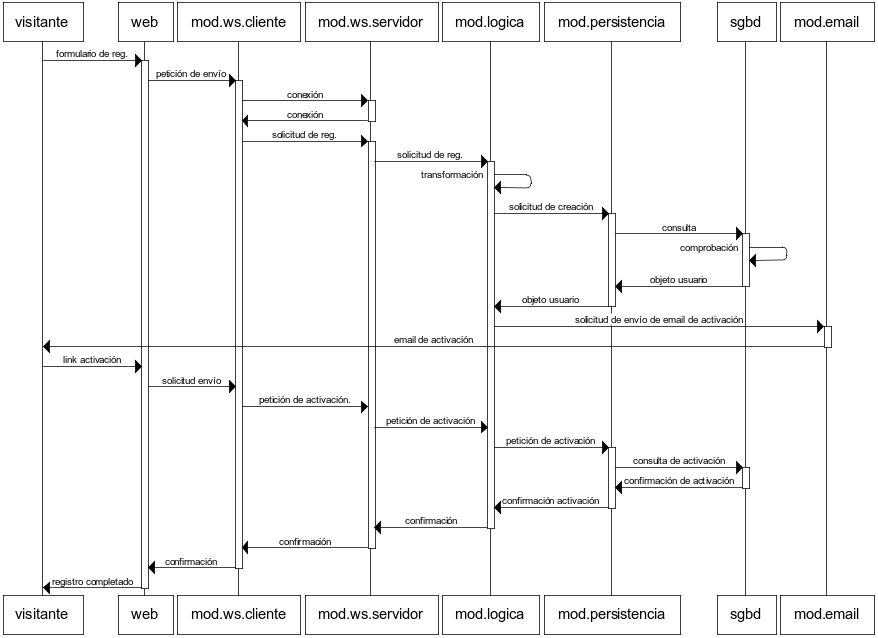
\includegraphics[width=\textwidth]{images/uc-3.png}
      \caption{Diagrama de interacción del caso de uso UC-3 (flujo normal)}
      \label{fig::uc-3}
    \end{center}
  \end{figure}

\item %%%%%%%%%%%%%%%%%%%%%%%%%%%%%%%%%%%%%%%%%%%%%%%%%%
  \begin{itemize}
  \item \textbf{Caso de uso}: Recuperar contraseña
  \item \textbf{Requisito funcional asociado}: RF-15
  \item \textbf{Actores}
    \begin{itemize}
    \item Usuario
    \item SGBD
    \end{itemize}
  \item \textbf{Descripción}: El usuario que olvidó su contraseña genera una nueva, sustituyendo ésta a la anterior.
  \item \textbf{Precondiciones}
    \begin{itemize}
    \item La persona no debe tener una sesión iniciada.
    \end{itemize}
  \item \textbf{Postcondiciones}
    \begin{itemize}
    \item La contraseña anterior del usuario queda sustituida por la nueva.
    \end{itemize}
  \item \textbf{Flujo normal}
    \begin{enumerate}
    \item El usuario hace clic sobre el enlace de recuperación de contraseña.
    \item La web le ofrece un diálogo para que introduzca el email con el que se registró.
    \item El usuario escribe su email y acepta el envío de un enlace para generar la contraseña.
    \item La web envía la solicitud al módulo de websockets cliente.
    \item El módulo cliente de websockets envía la solicitud al módulo servidor de websockets.
    \item El módulo servidor de websockets recibe la solicitud y la pasa al módulo de lógica del servidor.
    \item El módulo de lógica pasa la solicitud al módulo de persistencia.
    \item El módulo de persistencia pide el hash del objeto usuario asociado al email de la petición al SGBD.
    \item El SGBD devuelve el hash del usuario asociado al email.
    \item El módulo de persistencia devuelve el hash al módulo de lógica.
    \item El módulo de lógica genera un link y solicita al módulo de email el envío del mismo.
    \item El módulo de email envía el link a la dirección proporcionada por el usuario.
    \item El usuario sigue el enlace recibido por email y accede a la pantalla de generación de contraseña. Crea una nueva contraseña y acepta su envío.
    \item La web envía los nuevos datos al módulo cliente de websockets.
    \item El módulo cliente de websockets recibe la información y envía la solicitud de cambio de contraseña al módulo servidor de websockets.
    \item El módulo servidor de websockets pasa la petición al módulo de lógica del servidor.
    \item El módulo de lógica solicita la sobreescritura de la contraseña antigua al módulo de persistencia, y genera un hash nuevo para sobreescribir al antiguo y evitar que el link de regeneración de contraseña vuelva a usarse.
    \item El módulo de persistencia realiza las consultas pertinentes sobre el SGBD.
    \item El SGBD modifica los datos y devuelve una confirmación de que los cambios se han realizado satisfactoriamente.
    \item El módulo de persistencia devuelve la confirmación al módulo de lógica.
    \item El módulo de lógica solicita el envío de la confirmación al módulo servidor de websockets.
    \item El módulo servidor de websockets envía la confirmación al módulo cliente de websockets.
    \item El módulo cliente de websockets pasa la confirmación a la web.
    \item La web muestra un mensaje de éxito.
    \end{enumerate}
  \item \textbf{Includes}
    \begin{itemize}
    \item Ninguno
    \end{itemize}
  \item \textbf{Extensiones}
    \begin{itemize}
    \item Ninguna
    \end{itemize}
  \item \textbf{Diagrama de interacción}: Figura \ref{fig::uc-4}
  \end{itemize}
  
  \begin{figure}[h]
    \begin{center}
      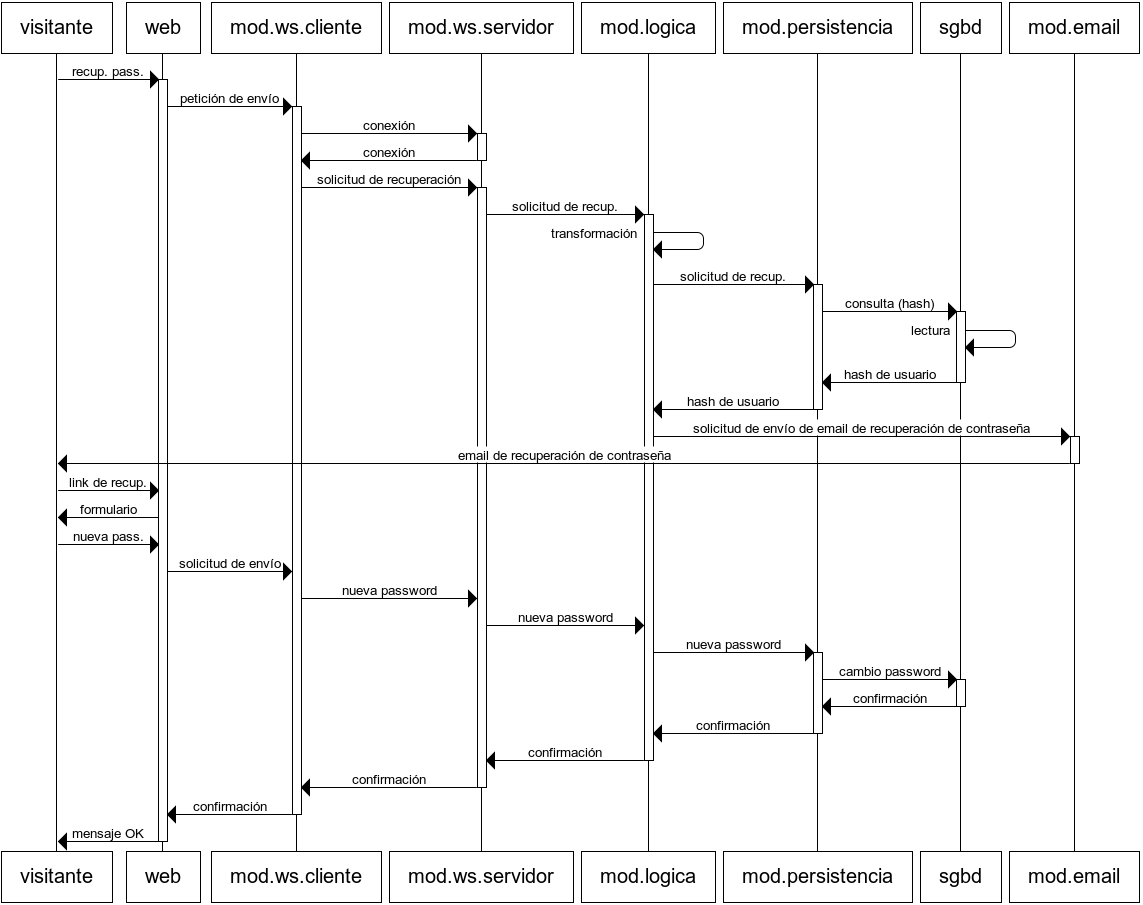
\includegraphics[width=\textwidth]{images/uc-4.png}
      \caption{Diagrama de interacción del caso de uso UC-4 (flujo normal)}
      \label{fig::uc-4}
    \end{center}
  \end{figure}

\item %%%%%%%%%%%%%%%%%%%%%%%%%%%%%%%%%%%%%%%%%%%%%%%%%%
  \begin{itemize}
  \item \textbf{Caso de uso}: Ver perfil
  \item \textbf{Requisitos funcionales asociados}: RF-16, RF-17
  \item \textbf{Actores}
    \begin{itemize}
    \item Usuario
    \item SGBD
    \end{itemize}
  \item \textbf{Descripción}: Un usuario solicita ver su perfil completo.
  \item \textbf{Precondiciones}
    \begin{itemize}
    \item El usuario está autenticado en el sistema
    \end{itemize}
  \item \textbf{Postcondiciones}
    \begin{itemize}
    \item Ninguna
    \end{itemize}
  \item \textbf{Flujo normal}
    \begin{enumerate}
    \item El usuario accede a la página de perfil.
    \item La web envía la petición de información al módulo cliente de websockets.
    \item El módulo cliente de websockets envía la petición al módulo servidor de websockets.
    \item El módulo servidor de websockets pasa la solicitud del perfil al módulo de lógica.
    \item El módulo de lógica del servidor pasa la solicitud al módulo de persistencia.
    \item El módulo de persistencia realiza una consulta sobre SGBD para recuperar el perfil de usuario.
    \item El SGBD recupera la información y se la envía de vuelta al módulo de persistencia.
    \item El módulo de persistencia devuelve el objeto de perfil al módulo de lógica.
    \item El módulo de lógica solicita el envío del perfil al módulo servidor de websockets.
    \item El módulo servidor de websockets envía la información al módulo cliente de websockets.
    \item El módulo cliente de websockets pasa toda la información de perfil a la web.
    \item La web se actualiza con la información del perfil completo.
    \end{enumerate}
  \item \textbf{Includes}
    \begin{itemize}
    \item Ninguno
    \end{itemize}
  \item \textbf{Extensiones}
    \begin{itemize}
    \item UC-6
    \end{itemize}
  \end{itemize}

\item %%%%%%%%%%%%%%%%%%%%%%%%%%%%%%%%%%%%%%%%%%%%%%%%%%
  \begin{itemize}
  \item \textbf{Caso de uso}: Editar perfil
  \item \textbf{Requisitos funcionales asociados}: RF-17
  \item \textbf{Actores}
    \begin{itemize}
    \item Usuario
    \item SGBD
    \end{itemize}
  \item \textbf{Descripción}: 
  \item \textbf{Precondiciones}
    \begin{itemize}
    \item El usuario está autenticado en el sistema.
    \end{itemize}
  \item \textbf{Postcondiciones}
    \begin{itemize}
    \item El perfil del usuario es modificado en la base de datos.
    \end{itemize}
  \item \textbf{Flujo normal}
    \begin{enumerate}
    \item El usuario accede a la página de perfil.
    \item La web envía la petición de información al módulo cliente de websockets.
    \item El módulo cliente de websockets envía la petición al módulo servidor de websockets.
    \item El módulo servidor de websockets pasa la solicitud del perfil al módulo de lógica.
    \item El módulo de lógica del servidor pasa la solicitud al módulo de persistencia.
    \item El módulo de persistencia realiza una consulta sobre SGBD para recuperar el perfil de usuario.
    \item El SGBD recupera la información y se la envía de vuelta al módulo de persistencia.
    \item El módulo de persistencia devuelve el objeto de perfil al módulo de lógica.
    \item El módulo de lógica solicita el envío del perfil al módulo servidor de websockets.
    \item El módulo servidor de websockets envía la información al módulo cliente de websockets.
    \item El módulo cliente de websockets pasa toda la información de perfil a la web.
    \item La web se actualiza con la información del perfil completo.
    \item El usuario modifica la información personal y pulsa el botón de guardar cambios.
    \item La web envía la solicitud de modificación al módulo cliente de websockets.
    \item El módulo cliente de websockets envía la solicitud al módulo servidor de websockets.
    \item El módulo servidor de websockets pasa la solicitud de modificación de perfil al módulo de lógica.
    \item El módulo de lógica pasa la solicitud al módulo de persistencia.
    \item El módulo de persistencia ejecuta las consultas de modificación sobre el SGBD.
    \item El SGBD devuelve una confirmación.
    \item El módulo de persistencia devuelve la confirmación al módulo de lógica.
    \item El módulo de lógica devuelve la confirmación al módulo servidor de websockets.
    \item El módulo servidor de websockets envía la confirmación al módulo cliente de websockets.
    \item El módulo cliente de websockets devuelve la confirmación a la web.
    \item La web se actualiza mostrando un mensaje de éxito al guardar los cambios.
    \end{enumerate}
  \item \textbf{Includes}
    \begin{itemize}
    \item Ninguno
    \end{itemize}
  \item \textbf{Extensiones}
    \begin{itemize}
    \item UC-8
    \item UC-7
    \end{itemize}
  \end{itemize}

\item %%%%%%%%%%%%%%%%%%%%%%%%%%%%%%%%%%%%%%%%%%%%%%%%%%
  \begin{itemize}
  \item \textbf{Caso de uso}: Modificar intereses
  \item \textbf{Requisitos funcionales asociados}: RF-16
  \item \textbf{Actores}
    \begin{itemize}
    \item Usuario
    \item SGBD
    \end{itemize}
  \item \textbf{Descripción}: El usuario modifica las habilidades mentales que quiere trabajar.
  \item \textbf{Precondiciones}
    \begin{itemize}
    \item El usuario debe estar autenticado en el sistema.
    \item El usuario debe estar visualizando su perfil.
    \end{itemize}
  \item \textbf{Postcondiciones}
    \begin{itemize}
    \item Los parámetros de entrenamiento cerebral (intereses mentales del usuario) se ven modificados de forma temporal (no permanente)
    \end{itemize}
  \item \textbf{Flujo normal}
    \begin{enumerate}
    \item El usuario hace clic sobre un botón para ver sus intereses actuales.
    \item La web solicita la información de intereses al módulo cliente de websockets.
    \item El módulo cliente de websockets envía la solicitud al módulo servidor de websockets.
    \item El módulo servidor de websockets recibe la petición y se la pasa al módulo de lógica del servidor.
    \item El módulo de lógica solicita la información al módulo de persistencia.
    \item El módulo de persistencia ejecuta la consulta de recuperación de intereses sobre el SGBD.
    \item El SGBD obtiene la información requerida y se la envía de vuelta al módulo de persistencia.
    \item El módulo de persistencia pasa la información de intereses al módulo de lógica.
    \item El módulo de lógica devuelve los datos al módulo servidor de websockets para que los envíe al cliente.
    \item El módulo servidor de websockets envía de vuelta la información al módulo cliente de websockets.
    \item El módulo cliente de websockets pasa la información a la web.
    \item La web muestra los intereses del usuario.
    \item El usuario modifica esos intereses.
    \end{enumerate}
  \item \textbf{Includes}
    \begin{itemize}
    \item Ninguno
    \end{itemize}
  \item \textbf{Extensiones}
    \begin{itemize}
    \item Ninguna
    \end{itemize}
  \end{itemize}

\item %%%%%%%%%%%%%%%%%%%%%%%%%%%%%%%%%%%%%%%%%%%%%%%%%%
  \begin{itemize}
  \item \textbf{Caso de uso}: Cambiar avatar
  \item \textbf{Requisitos funcionales asociados}: RF-18
  \item \textbf{Actores}
    \begin{itemize}
    \item Usuario
    \end{itemize}
  \item \textbf{Descripción}: El usuario modifica su avatar (imagen representativa).
  \item \textbf{Precondiciones}
    \begin{itemize}
    \item El usuario debe estar autenticado.
    \item El usuario debe encontrarse en la página de perfil.
    \end{itemize}
  \item \textbf{Postcondiciones}
    \begin{itemize}
    \item El avatar de usuario es cambiado de forma temporal (no permanente).
    \end{itemize}
  \item \textbf{Flujo normal}
    \begin{enumerate}
    \item El usuario hace clic sobre un botón para ``cambiar su avatar''.
    \item La web le muestra un mensaje de diálogo para que seleccione una imagen nueva desde su ordenador.
    \item El usuario selecciona una imagen y acepta.
    \item La web recupera la imagen elegida y sustituye al avatar anterior.
    \end{enumerate}
  \item \textbf{Includes}
    \begin{itemize}
    \item Ninguno
    \end{itemize}
  \item \textbf{Extensiones}
    \begin{itemize}
    \item Ninguna
    \end{itemize}
  \end{itemize}

\item %%%%%%%%%%%%%%%%%%%%%%%%%%%%%%%%%%%%%%%%%%%%%%%%%%
  \begin{itemize}
  \item \textbf{Caso de uso}: Buscar usuarios
  \item \textbf{Requisitos funcionales asociados}: RF-24
  \item \textbf{Actores}
    \begin{itemize}
    \item Usuario
    \item SGBD
    \end{itemize}
  \item \textbf{Descripción}: El usuario ejecuta una búsqueda sobre el sistema, que le devuelve un listado de usuarios coincidentes con dicha consulta.
  \item \textbf{Precondiciones}
    \begin{itemize}
    \item El usuario debe estar autenticado en la web.
    \item El usuario se encuentra visualizando la página de exploración de usuarios.
    \end{itemize}
  \item \textbf{Postcondiciones}
    \begin{itemize}
    \item Ninguna
    \end{itemize}
  \item \textbf{Flujo normal}
    \begin{enumerate}
    \item El usuario rellena el formulario de búsqueda y hace clic sobre el botón de buscar.
    \item La web construye la estructura de datos adecuada para almacenar la información del formulario y solicita su envío al módulo cliente de websockets.
    \item El módulo cliente de websockets envía la información al módulo servidor de websockets.
    \item El módulo servidor de websockets pasa la información al módulo de lógica del servidor.
    \item El módulo de lógica pasa la información de búsqueda al módulo de persistencia.
    \item El módulo de persistencia ejecuta el algoritmo de búsqueda sobre el SGBD.
    \item El SGBD devuelve un listado de resultados coincidentes con la búsqueda.
    \item El módulo de persistencia devuelve los resultados al módulo de lógica del servidor.
    \item El módulo de lógica solicita el envío de los resultados al módulo servidor de websockets.
    \item El módulo servidor de websockets envía los resultados al módulo cliente de websockets.
    \item El módulo cliente de websockets recibe los resultados y se los pasa a la web.
    \item La web se actualiza y muestra los resultados de la búsqueda.
    \end{enumerate}
  \item \textbf{Includes}
    \begin{itemize}
    \item Ninguno
    \end{itemize}
  \item \textbf{Extensiones}
    \begin{itemize}
    \item UC-10
    \item UC-11
    \end{itemize}
  \end{itemize}

\item %%%%%%%%%%%%%%%%%%%%%%%%%%%%%%%%%%%%%%%%%%%%%%%%%%
  \begin{itemize}
  \item \textbf{Caso de uso}: Seguir a un usuario
  \item \textbf{Requisitos funcionales asociados}: RF-19
  \item \textbf{Actores}
    \begin{itemize}
    \item Usuario
    \item SGBD
    \end{itemize}
  \item \textbf{Descripción}: El usuario actual se convierte en seguidor de otro usuario.
  \item \textbf{Precondiciones}
    \begin{itemize}
    \item El usuario está autenticado en la web.
    \item El usuario se encuentra en la página de exploración de usuarios.
    \item El usuario ha realizado una búsqueda de usuarios cuyo resultado incluye al usuario objetivo.
    \item El usuario actual no es seguidor del usuario al que se va a empezar a seguir.
    \end{itemize}
  \item \textbf{Postcondiciones}
    \begin{itemize}
    \item El usuario actual es seguidor del otro usuario.
    \end{itemize}
  \item \textbf{Flujo normal}
    \begin{enumerate}
    \item El usuario hace clic sobre el resultado de búsqueda asociado al usuario objetivo.
    \item La web muestra el perfil del usuario objetivo.
    \item El usuario actual hace clic sobre el botón ``seguir''.
    \item La web envía la solicitud de seguimiento al módulo cliente de websockets.
    \item El módulo cliente de websockets envía la solicitud de seguimiento al módulo servidor de websockets.
    \item El módulo de lógica pasa la solicitud al módulo de persistencia.
    \item El módulo de persistencia ejecuta la consulta de establecimiento de un nuevo seguidor sobre el SGBD.
    \item El SGBD actualiza la base de datos y devuelve una confirmación.
    \item El módulo de persistencia devuelve la confirmación al módulo de lógica del servidor.
    \item El módulo de lógica solicita el envío de la confirmación al módulo servidor de websockets.
    \item El módulo servidor de websockets envía la confirmación al módulo cliente de websockets.
    \item El módulo cliente de websockets recibe la confirmación y se los pasa a la web.
    \item La web se actualiza y muestra un mensaje de éxito.
    \end{enumerate}
  \item \textbf{Includes}
    \begin{itemize}
    \item Ninguno
    \end{itemize}
  \item \textbf{Extensiones}
    \begin{itemize}
    \item Ninguna
    \end{itemize}
  \end{itemize}


\item %%%%%%%%%%%%%%%%%%%%%%%%%%%%%%%%%%%%%%%%%%%%%%%%%%
  \begin{itemize}
  \item \textbf{Caso de uso}: Dejar de seguir a un usuario
  \item \textbf{Requisitos funcionales asociados}: RF-20
  \item \textbf{Actores}
    \begin{itemize}
    \item Usuario
    \item SGBD
    \end{itemize}
  \item \textbf{Descripción}: El usuario actual deja de ser seguidor de otro usuario.
  \item \textbf{Precondiciones}
    \begin{itemize}
    \item El usuario está autenticado en la web.
    \item El usuario se encuentra en la página de exploración de usuarios.
    \item El usuario ha realizado una búsqueda de usuarios cuyo resultado incluye al usuario objetivo.
    \item El usuario actual es seguidor del usuario al que se va a dejar de seguir.
    \end{itemize}
  \item \textbf{Postcondiciones}
    \begin{itemize}
    \item El usuario actual no es seguidor del otro usuario.
    \end{itemize}
  \item \textbf{Flujo normal}
    \begin{enumerate}
    \item El usuario hace clic sobre el resultado de búsqueda asociado al usuario objetivo.
    \item La web muestra el perfil del usuario objetivo.
    \item El usuario actual hace clic sobre el botón ``dejar de seguir''.
    \item La web envía la solicitud de anulación de seguimiento al módulo cliente de websockets.
    \item El módulo cliente de websockets envía la solicitud de anulación de seguimiento al módulo servidor de websockets.
    \item El módulo de lógica pasa la solicitud al módulo de persistencia.
    \item El módulo de persistencia ejecuta la consulta de eliminación de un seguidor sobre el SGBD.
    \item El SGBD actualiza la base de datos y devuelve una confirmación.
    \item El módulo de persistencia devuelve la confirmación al módulo de lógica del servidor.
    \item El módulo de lógica solicita el envío de la confirmación al módulo servidor de websockets.
    \item El módulo servidor de websockets envía la confirmación al módulo cliente de websockets.
    \item El módulo cliente de websockets recibe la confirmación y se los pasa a la web.
    \item La web se actualiza y muestra un mensaje de éxito.
    \end{enumerate}
  \item \textbf{Includes}
    \begin{itemize}
    \item Ninguno
    \end{itemize}
  \item \textbf{Extensiones}
    \begin{itemize}
    \item Ninguna
    \end{itemize}
  \end{itemize}

\item %%%%%%%%%%%%%%%%%%%%%%%%%%%%%%%%%%%%%%%%%%%%%%%%%%
  \begin{itemize}
  \item \textbf{Caso de uso}: Jugar a un juego
  \item \textbf{Requisitos funcionales asociados}: RF-8, RF-27
  \item \textbf{Actores}
    \begin{itemize}
    \item Usuario
    \item SGBD
    \end{itemize}
  \item \textbf{Descripción}: El usuario lanza un juego para jugar a él.
  \item \textbf{Precondiciones}
    \begin{itemize}
    \item El usuario debe estar autenticado en el sistema.
    \end{itemize}
  \item \textbf{Postcondiciones}
    \begin{itemize}
    \item El perfil cerebral es actualizado con los resultados de la partida.
    \end{itemize}
  \item \textbf{Flujo normal}
    \begin{enumerate}
    \item El usuario accede a la página de juegos.
    \item La web solicita la petición de los listados de juegos al módulo cliente de websockets.
    \item El módulo cliente de websockets envía la solicitud al módulo servidor de websockets.
    \item El módulo servidor de websockets pasa la solicitud al módulo de lógica.
    \item El módulo de lógica realiza la petición al módulo de juegos.
    \item El módulo de juegos devuelve un listado con todos los juegos disponibles.
    \item El módulo de lógica solicita el envío del listado al módulo servidor de websockets.
    \item El módulo servidor de websockets envía el listado de juegos al módulo cliente de websockets.
    \item El módulo cliente de websockets devuelve el listado de juegos a la web.
    \item La web carga la página solicitada con los juegos disponibles.
    \item El usuario selecciona un juego al que jugar.
    \item La web solicita el juego al módulo cliente de websockets.
    \item El módulo cliente de websockets envía la petición al módulo servidor de websockets.
    \item El módulo servidor de websockets pasa la petición al módulo de lógica.
    \item El módulo de lógica solicita el juego pedido al módulo de juegos.
    \item El módulo de juegos devuelve el juego solicitado completo.
    \item El módulo de lógica solicita el envío del juego al módulo servidor de websockets.
    \item El módulo servidor de websockets envía el juego al módulo cliente de websockets.
    \item El módulo cliente de websockets pasa el juego a la web.
    \item La web carga el juego recibido y lo ejecuta.
    \end{enumerate}
  \item \textbf{Includes}
    \begin{itemize}
    \item UC-13
    \end{itemize}
  \item \textbf{Extensiones}
    \begin{itemize}
    \item Ninguna
    \end{itemize}
  \item \textbf{Diagrama de interacción}: Figura \ref{fig::uc-12}
  \end{itemize}


  \begin{figure}[h]
    \begin{center}
      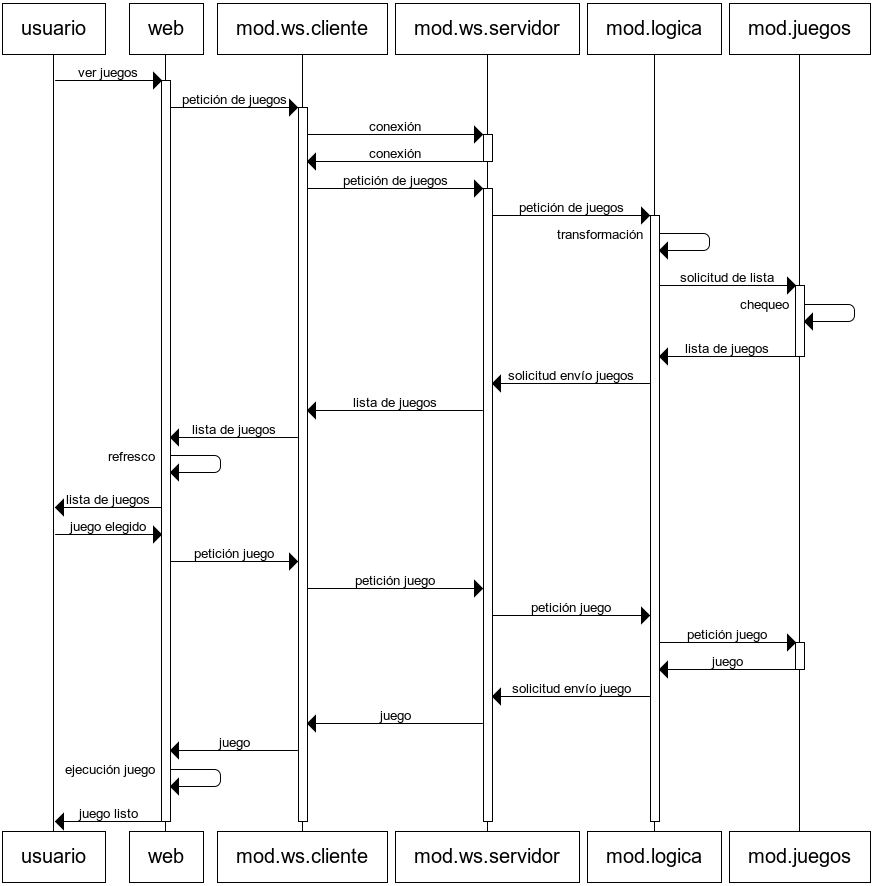
\includegraphics[width=\textwidth]{images/uc-12.png}
      \caption{Diagrama de interacción del caso de uso UC-12 (flujo normal)}
      \label{fig::uc-12}
    \end{center}
  \end{figure}
  


\item %%%%%%%%%%%%%%%%%%%%%%%%%%%%%%%%%%%%%%%%%%%%%%%%%%
  \begin{itemize}
  \item \textbf{Caso de uso}: Actualizar perfil cerebral
  \item \textbf{Requisitos funcionales asociados}: RF-8, RF-27
  \item \textbf{Actores}
    \begin{itemize}
    \item SGBD
    \end{itemize}
  \item \textbf{Descripción}: Tras una partida, el perfil cerebral es actualizado.
  \item \textbf{Precondiciones}
    \begin{itemize}
    \item El usuario está autenticado en el sistema.
    \item El usuario acaba de terminar una partida.
    \end{itemize}
  \item \textbf{Postcondiciones}
    \begin{itemize}
    \item El perfil cerebral del usuario queda modificado.
    \end{itemize}
  \item \textbf{Flujo normal}
    \begin{enumerate}
    \item La web solicita el envío del resultado al módulo cliente de websockets.
    \item El módulo cliente de websockets envía el resultado al módulo servidor de websockets.
    \item El módulo servidor de websockets pasa el resultado al módulo de lógica del servidor.
    \item El módulo de lógica solicita la actualización del perfil cerebral al módulo de persistencia.
    \item El módulo de persistencia ejecuta las consultas de actualización sobre el SGBD.
    \item El SGBD realiza la actualización del perfil cerebral y devuelve una confirmación al módulo de persistencia.
    \item El módulo de persistencia devuelve la confirmación al módulo de lógica.
    \item El módulo de lógica solicita el envío de la confirmación al módulo servidor de websockets.
    \item El módulo servidor de websockets envía la confirmación al módulo cliente de websockets.
    \item El módulo cliente de websockets pasa la confirmación a la web.
    \item La web muestra una notificación confirmando que el perfil cerebral ha sido actualizado.
    \end{enumerate}
  \item \textbf{Includes}
    \begin{itemize}
    \item Ninguno
    \end{itemize}
  \item \textbf{Extensiones}
    \begin{itemize}
    \item Ninguna
    \end{itemize}
  \end{itemize}

\item %%%%%%%%%%%%%%%%%%%%%%%%%%%%%%%%%%%%%%%%%%%%%%%%%%
  \begin{itemize}
  \item \textbf{Caso de uso}: Jugar a un juego monojugador
  \item \textbf{Requisitos funcionales asociados}: RF-8, RF-27
  \item \textbf{Actores}
    \begin{itemize}
    \item Usuario
    \item SGBD
    \end{itemize}
  \item \textbf{Descripción}: 
  \item \textbf{Precondiciones}
    \begin{itemize}
    \item El usuario debe estar autenticado en el sistema
    \item El usuario debe estar situado en la página de juegos, con el listado cargado.
    \end{itemize}
  \item \textbf{Postcondiciones}
    \begin{itemize}
    \item Ninguna
    \end{itemize}
  \item \textbf{Flujo normal}
    \begin{enumerate}
    \item El usuario selecciona un juego monojugador al que jugar.
    \item La web solicita el juego al módulo cliente de websockets.
    \item El módulo cliente de websockets envía la petición al módulo servidor de websockets.
    \item El módulo servidor de websockets pasa la petición al módulo de lógica.
    \item El módulo de lógica solicita el juego pedido al módulo de juegos.
    \item El módulo de juegos devuelve el juego solicitado completo.
    \item El módulo de lógica solicita el envío del juego al módulo servidor de websockets.
    \item El módulo servidor de websockets envía el juego al módulo cliente de websockets.
    \item El módulo cliente de websockets pasa el juego a la web.
    \item La web carga el juego recibido y lo ejecuta.
    \end{enumerate}
  \item \textbf{Includes}
    \begin{itemize}
    \item Ninguno
    \end{itemize}
  \item \textbf{Extensiones}
    \begin{itemize}
    \item UC-15
    \end{itemize}
  \item \textbf{Generalización de}: UC-12
  \end{itemize}

\item %%%%%%%%%%%%%%%%%%%%%%%%%%%%%%%%%%%%%%%%%%%%%%%%%%
  \begin{itemize}
  \item \textbf{Caso de uso}: Recomendar juego
  \item \textbf{Requisitos funcionales asociados}: RF-8, RF-27, RF-25
  \item \textbf{Actores}
    \begin{itemize}
    \item Usuario
    \item SGBD
    \end{itemize}
  \item \textbf{Descripción}: El usuario recomienda un juego monojugador a otro usuario.
  \item \textbf{Precondiciones}
    \begin{itemize}
    \item El usuario está autenticado en el sistema.
    \item El usuario ha cargado un juego.
    \end{itemize}
  \item \textbf{Postcondiciones}
    \begin{itemize}
    \item El usuario destino de la recomendación recibe una notificación por email.
    \end{itemize}
  \item \textbf{Flujo normal}
    \begin{enumerate}
    \item El usuario pulsa el botón de ``recomendar'' junto a un juego cargado, y selecciona un usuario al que enviar dicha recomendación.
    \item La web solicita el envío de la recomendación al módulo cliente de websockets.
    \item El módulo cliente de websockets envía la petición de recomendación al módulo servidor de websockets.
    \item El módulo servidor de websockets pasa la petición de recomendación al módulo de lógica.
    \item El módulo de lógica solicita los datos de contacto del usuario destino de la recomendación al módulo de persistencia.
    \item El módulo de persistencia realiza una consulta para recuperar la información del usuario destino de la recomendación al SGBD.
    \item El SGBD recupera la información y la envía de vuelta al módulo de persistencia.
    \item El módulo de persistencia pasa los datos de contacto al módulo de lógica.
    \item El módulo de lógica solicita el envío de la recomendación al módulo de email.
    \item El módulo de email envía la recomendación al usuario correspondiente, y devuelve una confirmación al módulo de lógica.
    \item El módulo de lógica solicita el envío de la confirmación de vuelta al cliente al módulo servidor de websockets.
    \item El módulo servidor de websockets envía la confirmación de recomendación al módulo cliente de websockets.
    \item El módulo cliente de websockets pasa la confirmación a la web.
    \item La web muestra una notificación informando de que la recomendación ha sido enviada correctamente.
    \end{enumerate}
  \item \textbf{Includes}
    \begin{itemize}
    \item Ninguno
    \end{itemize}
  \item \textbf{Extensiones}
    \begin{itemize}
    \item Ninguna
    \end{itemize}
  \end{itemize}


\item %%%%%%%%%%%%%%%%%%%%%%%%%%%%%%%%%%%%%%%%%%%%%%%%%%
  \begin{itemize}
  \item \textbf{Caso de uso}: Jugar a un juego multijugador
  \item \textbf{Requisitos funcionales asociados}: RF-8, RF-27
  \item \textbf{Actores}
    \begin{itemize}
    \item Usuario
    \item SGBD
    \end{itemize}
  \item \textbf{Descripción}: 
  \item \textbf{Precondiciones}
    \begin{itemize}
    \item El usuario debe estar autenticado en el sistema.
    \item El usuario debe estar situado en la página de juegos, con el listado cargado.
    \end{itemize}
  \item \textbf{Postcondiciones}
    \begin{itemize}
    \item El perfil cerebral de ambos jugadores se ve modificado.
    \end{itemize}
  \item \textbf{Flujo normal}
    \begin{enumerate}
    \item El usuario selecciona un juego multijugador al que jugar y un usuario contra el que jugar.
    \item La web solicita el juego y el envío de la invitación al módulo cliente de websockets.
    \item El módulo cliente de websockets envía la petición al módulo servidor de websockets.
    \item El módulo servidor de websockets pasa la petición al módulo de lógica.
    \item El módulo de lógica solicita el envío de la invitación al módulo servidor de websockets.
    \item El módulo servidor de websockets envía la invitación al módulo cliente de websockets del otro usuario (el retado).
    \item El módulo cliente de websockets del usuario retado pasa la invitación a la web.
    \item La web muestra la invitación y permite aceptarla o rechazarla.
    \item El usuario retado acepta la invitación.
    \item La web envía el mensaje de aceptación al módulo cliente de websockets.
    \item El módulo cliente de websockets  del usuario retado envía el mensaje de aceptación al módulo servidor de websockets.
    \item El módulo servidor de websockets pasa el mensaje de aceptación al módulo de lógica.
    \item El módulo de lógica solicita el juego pedido al módulo de juegos.
    \item El módulo de juegos devuelve el juego solicitado completo.
    \item El módulo de lógica solicita el envío del juego al módulo servidor de websockets.
    \item El módulo servidor de websockets envía el juego al módulo cliente de websockets de cada usuario.
    \item El módulo cliente de websockets pasa el juego a la web.
    \item La web carga el juego recibido y lo ejecuta.    
    \end{enumerate}
  \item \textbf{Flujo alternativo 1}: El usuario retado rechaza la invitación a jugar
    \begin{enumerate}
    \item El usuario selecciona un juego multijugador al que jugar y un usuario contra el que jugar.
    \item La web solicita el juego y el envío de la invitación al módulo cliente de websockets.
    \item El módulo cliente de websockets envía la petición al módulo servidor de websockets.
    \item El módulo servidor de websockets pasa la petición al módulo de lógica.
    \item El módulo de lógica solicita el envío de la invitación al módulo servidor de websockets.
    \item El módulo servidor de websockets envía la invitación al módulo cliente de websockets del otro usuario (el retado).
    \item El módulo cliente de websockets del usuario retado pasa la invitación a la web.
    \item La web muestra la invitación y permite aceptarla o rechazarla.
    \item El usuario retado rechaza la invitación.
    \item La web envía el mensaje de rechazo al módulo cliente de websockets.
    \item El módulo cliente de websockets del usuario retado envía el mensaje de rechazo al módulo servidor de websockets.
    \item El módulo servidor de websockets pasa el mensaje de rechazo al módulo de lógica.
    \item El módulo de lógica solicita el envío de rechazo al módulo servidor de websockets.
    \item El módulo servidor de websockets envía el rechazo al módulo cliente de websockets del usuario original.
    \item El módulo cliente de websockets pasa el mensaje de rechazo a la web.
    \item La web notifica el rechazo del reto.
    \end{enumerate}
  \item \textbf{Includes}
    \begin{itemize}
    \item Ninguno
    \end{itemize}
  \item \textbf{Extensiones}
    \begin{itemize}
    \item UC-18
    \item UC-19
    \end{itemize}
  \item \textbf{Generalización de}: UC-12
  \end{itemize}


\item %%%%%%%%%%%%%%%%%%%%%%%%%%%%%%%%%%%%%%%%%%%%%%%%%%
  \begin{itemize}
  \item \textbf{Caso de uso}: Ver recomendaciones de juegos
  \item \textbf{Requisitos funcionales asociados}: RF-8, RF-27, RF-25
  \item \textbf{Actores}
    \begin{itemize}
    \item Usuario
    \item SGBD
    \end{itemize}
  \item \textbf{Descripción}: El usuario recibe recomendaciones automatizadas de juegos por parte del sistema de recomendación.
  \item \textbf{Precondiciones}
    \begin{itemize}
    \item El usuario está autenticado en el sistema.
    \end{itemize}
  \item \textbf{Postcondiciones}
    \begin{itemize}
    \item Ninguna
    \end{itemize}
  \item \textbf{Flujo normal}
    \begin{enumerate}
    \item El usuario accede a la página de juegos.
    \item La web solicita la recomendación de juegos al módulo cliente de websockets.
    \item El módulo cliente de websockets envía la petición al módulo servidor de websockets.
    \item El módulo servidor de websockets pasa la petición de recomendación al módulo de lógica.
    \item El módulo de lógica solicita el listado de juegos al módulo de juegos.
    \item El módulo de juegos devuelve al módulo de lógica el listado de juegos disponibles.
    \item El módulo de lógica solicita la información completa del usuario al módulo de persistencia.
    \item El módulo de persistencia lanza una consulta al SGBD para recuperar la información del usuario.
    \item El SGBD devuelve la información completa del usuario al módulo de persistencia.
    \item El módulo de persistencia pasa los datos del usuario al módulo de lógica.
    \item El módulo de lógica solicita la recomendación de juegos al módulo de recomendación, adjuntándole el listado de juegos y la información completa del usuario.
    \item El módulo de recomendación devuelve el resultado del algoritmo de recomendación de juegos al módulo de lógica.
    \item El módulo de lógica solicita el envío de la recomendación al módulo servidor de websockets.
    \item El módulo servidor de websockets envía la recomendación al módulo cliente de websockets.
    \item El módulo cliente de websockets pasa la recomendación a la web.
    \item La web muestra los resultados de la recomendación en la página de juegos.
    \end{enumerate}
  \item \textbf{Includes}
    \begin{itemize}
    \item Ninguno
    \end{itemize}
  \item \textbf{Extensiones}
    \begin{itemize}
    \item Ninguna
    \end{itemize}
  \end{itemize}

% \item %%%%%%%%%%%%%%%%%%%%%%%%%%%%%%%%%%%%%%%%%%%%%%%%%%
%   \begin{itemize}
%   \item \textbf{Caso de uso}: Retar a otro usuario
%   \item \textbf{Requisitos funcionales asociados}: RF-8, RF-27, RF-28
%   \item \textbf{Actores}
%     \begin{itemize}
%     \item Usuario
%     \item SGBD
%     \end{itemize}
%   \item \textbf{Descripción}: 
%   \item \textbf{Precondiciones}
%     \begin{itemize}
%     \item 
%     \end{itemize}
%   \item \textbf{Postcondiciones}
%     \begin{itemize}
%     \item 
%     \end{itemize}
%   \item \textbf{Flujo normal}
%     \begin{enumerate}
%     \item 
%     \end{enumerate}
%   \item \textbf{Includes}
%     \begin{itemize}
%     \item Ninguno
%     \end{itemize}
%   \item \textbf{Extensiones}
%     \begin{itemize}
%     \item Ninguna
%     \end{itemize}
%   \item \textbf{Diagrama de interacción}: Figura 
%   \end{itemize}


% \item %%%%%%%%%%%%%%%%%%%%%%%%%%%%%%%%%%%%%%%%%%%%%%%%%%
%   \begin{itemize}
%   \item \textbf{Caso de uso}: Aceptar reto de juego
%   \item \textbf{Requisitos funcionales asociados}: RF-8, RF-27, RF-28
%   \item \textbf{Actores}
%     \begin{itemize}
%     \item Usuario
%     \item SGBD
%     \end{itemize}
%   \item \textbf{Descripción}: 
%   \item \textbf{Precondiciones}
%     \begin{itemize}
%     \item 
%     \end{itemize}
%   \item \textbf{Postcondiciones}
%     \begin{itemize}
%     \item 
%     \end{itemize}
%   \item \textbf{Flujo normal}
%     \begin{enumerate}
%     \item 
%     \end{enumerate}
%   \item \textbf{Includes}
%     \begin{itemize}
%     \item Ninguno
%     \end{itemize}
%   \item \textbf{Extensiones}
%     \begin{itemize}
%     \item Ninguna
%     \end{itemize}
%   \item \textbf{Diagrama de interacción}: Figura 
%   \end{itemize}

\item %%%%%%%%%%%%%%%%%%%%%%%%%%%%%%%%%%%%%%%%%%%%%%%%%%
  \begin{itemize}
  \item \textbf{Caso de uso}: Ver recomendaciones de usuarios
  \item \textbf{Requisitos funcionales asociados}: RF-26
  \item \textbf{Actores}
    \begin{itemize}
    \item Usuario
    \item SGBD
    \end{itemize}
  \item \textbf{Descripción}: El usuario recibe recomendaciones automatizadas de usuarios similares a él por parte del sistema de recomendación.
  \item \textbf{Precondiciones}
    \begin{itemize}
    \item El usuario está autenticado en el sistema.
    \end{itemize}
  \item \textbf{Postcondiciones}
    \begin{itemize}
    \item Ninguna
    \end{itemize}
  \item \textbf{Flujo normal}
    \begin{enumerate}
    \item El usuario accede a la página de exploración de usuarios.
    \item La web solicita la recomendación de usuarios al módulo cliente de websockets.
    \item El módulo cliente de websockets envía la petición al módulo servidor de websockets.
    \item El módulo servidor de websockets pasa la petición de recomendación al módulo de lógica.
    \item El módulo de lógica solicita el listado de usuarios al módulo de persistencia.
    \item El módulo de persistencia lanza una consulta de usuarios al SGBD.
    \item El SGBD devuelve un listado acotado de usuarios.
    \item El módulo de persistencia devuelve al módulo de lógica el listado de usuarios.
    \item El módulo de lógica solicita la información completa del usuario al módulo de persistencia.
    \item El módulo de persistencia lanza una consulta al SGBD para recuperar la información del usuario.
    \item El SGBD devuelve la información completa del usuario al módulo de persistencia.
    \item El módulo de persistencia pasa los datos del usuario al módulo de lógica.
    \item El módulo de lógica solicita la recomendación de usuarios al módulo de recomendación, adjuntándole el listado de usuarios y la información completa del usuario.
    \item El módulo de recomendación devuelve el resultado del algoritmo de recomendación de usuarios al módulo de lógica.
    \item El módulo de lógica solicita el envío de la recomendación al módulo servidor de websockets.
    \item El módulo servidor de websockets envía la recomendación al módulo cliente de websockets.
    \item El módulo cliente de websockets pasa la recomendación a la web.
    \item La web muestra los resultados de la recomendación en la página de usuarios.
    \end{enumerate}
  \item \textbf{Includes}
    \begin{itemize}
    \item Ninguno
    \end{itemize}
  \item \textbf{Extensiones}
    \begin{itemize}
    \item Ninguna
    \end{itemize}
  \end{itemize}








\end{enumerate}






\section{Diseño}

Dada la naturaleza de la tecnología empleada para el desarrollo del sistema de BreakBrain, la implementación se lleva a cabo de forma modular sobre el núcleo que supone NodeJS\index{nodejs} ---en el lado del servidor---. Tanto a ese nivel como en el lado del cliente, se sigue el patrón MVC para la construcción del software.

En cuanto al servidor, las tres capas MVC son las siguientes:

\begin{itemize}
\item {\bf Servidor web / Servidor de websockets}: Se encarga de la comunicación con el sistema cliente. Actúa como intermediario entre éste y el núcleo del servidor, en el que se implementa la lógica principal del sistema.
\item {\bf Núcleo del servidor}: Se trata de la lógica de dominio, donde se codifica el comportamiento central de BreakBrain, en torno al cual se presentan el resto de componentes software.
\item {\bf Subsistema de persistencia}: Es el responsable del almacenamiento y recuperación de la información referida a los usuarios y las partidas, los perfiles de evolución cerebral, etc. Se comunica con el núcleo del servidor y actúa de intermediario entre éste y el \acf{SGBD}, que es proporcionado por un servicio remoto.
\end{itemize}

Atendiendo al cliente, las capas MVC en las que se divide su implementación son las enumeradas a continuación:

\begin{itemize}
\item {\bf Web (GUI)}: Se trata de la capa de presentación, a través de la cual el usuario interactúa con el sistema. Éste es el único componente software del cual el usuario final tiene constancia.
\item {\bf Lógica del cliente}: Esta capa manipula la información del usuario y actúa de intermediaria entre la interfaz gráfica (web) y la capa de persistencia temporal del cliente.
\item {\bf Persistencia temporal}: Se encarga de mantener la sesión temporal del usuario.
\end{itemize}

\begin{figure}[h]
  \begin{center}
    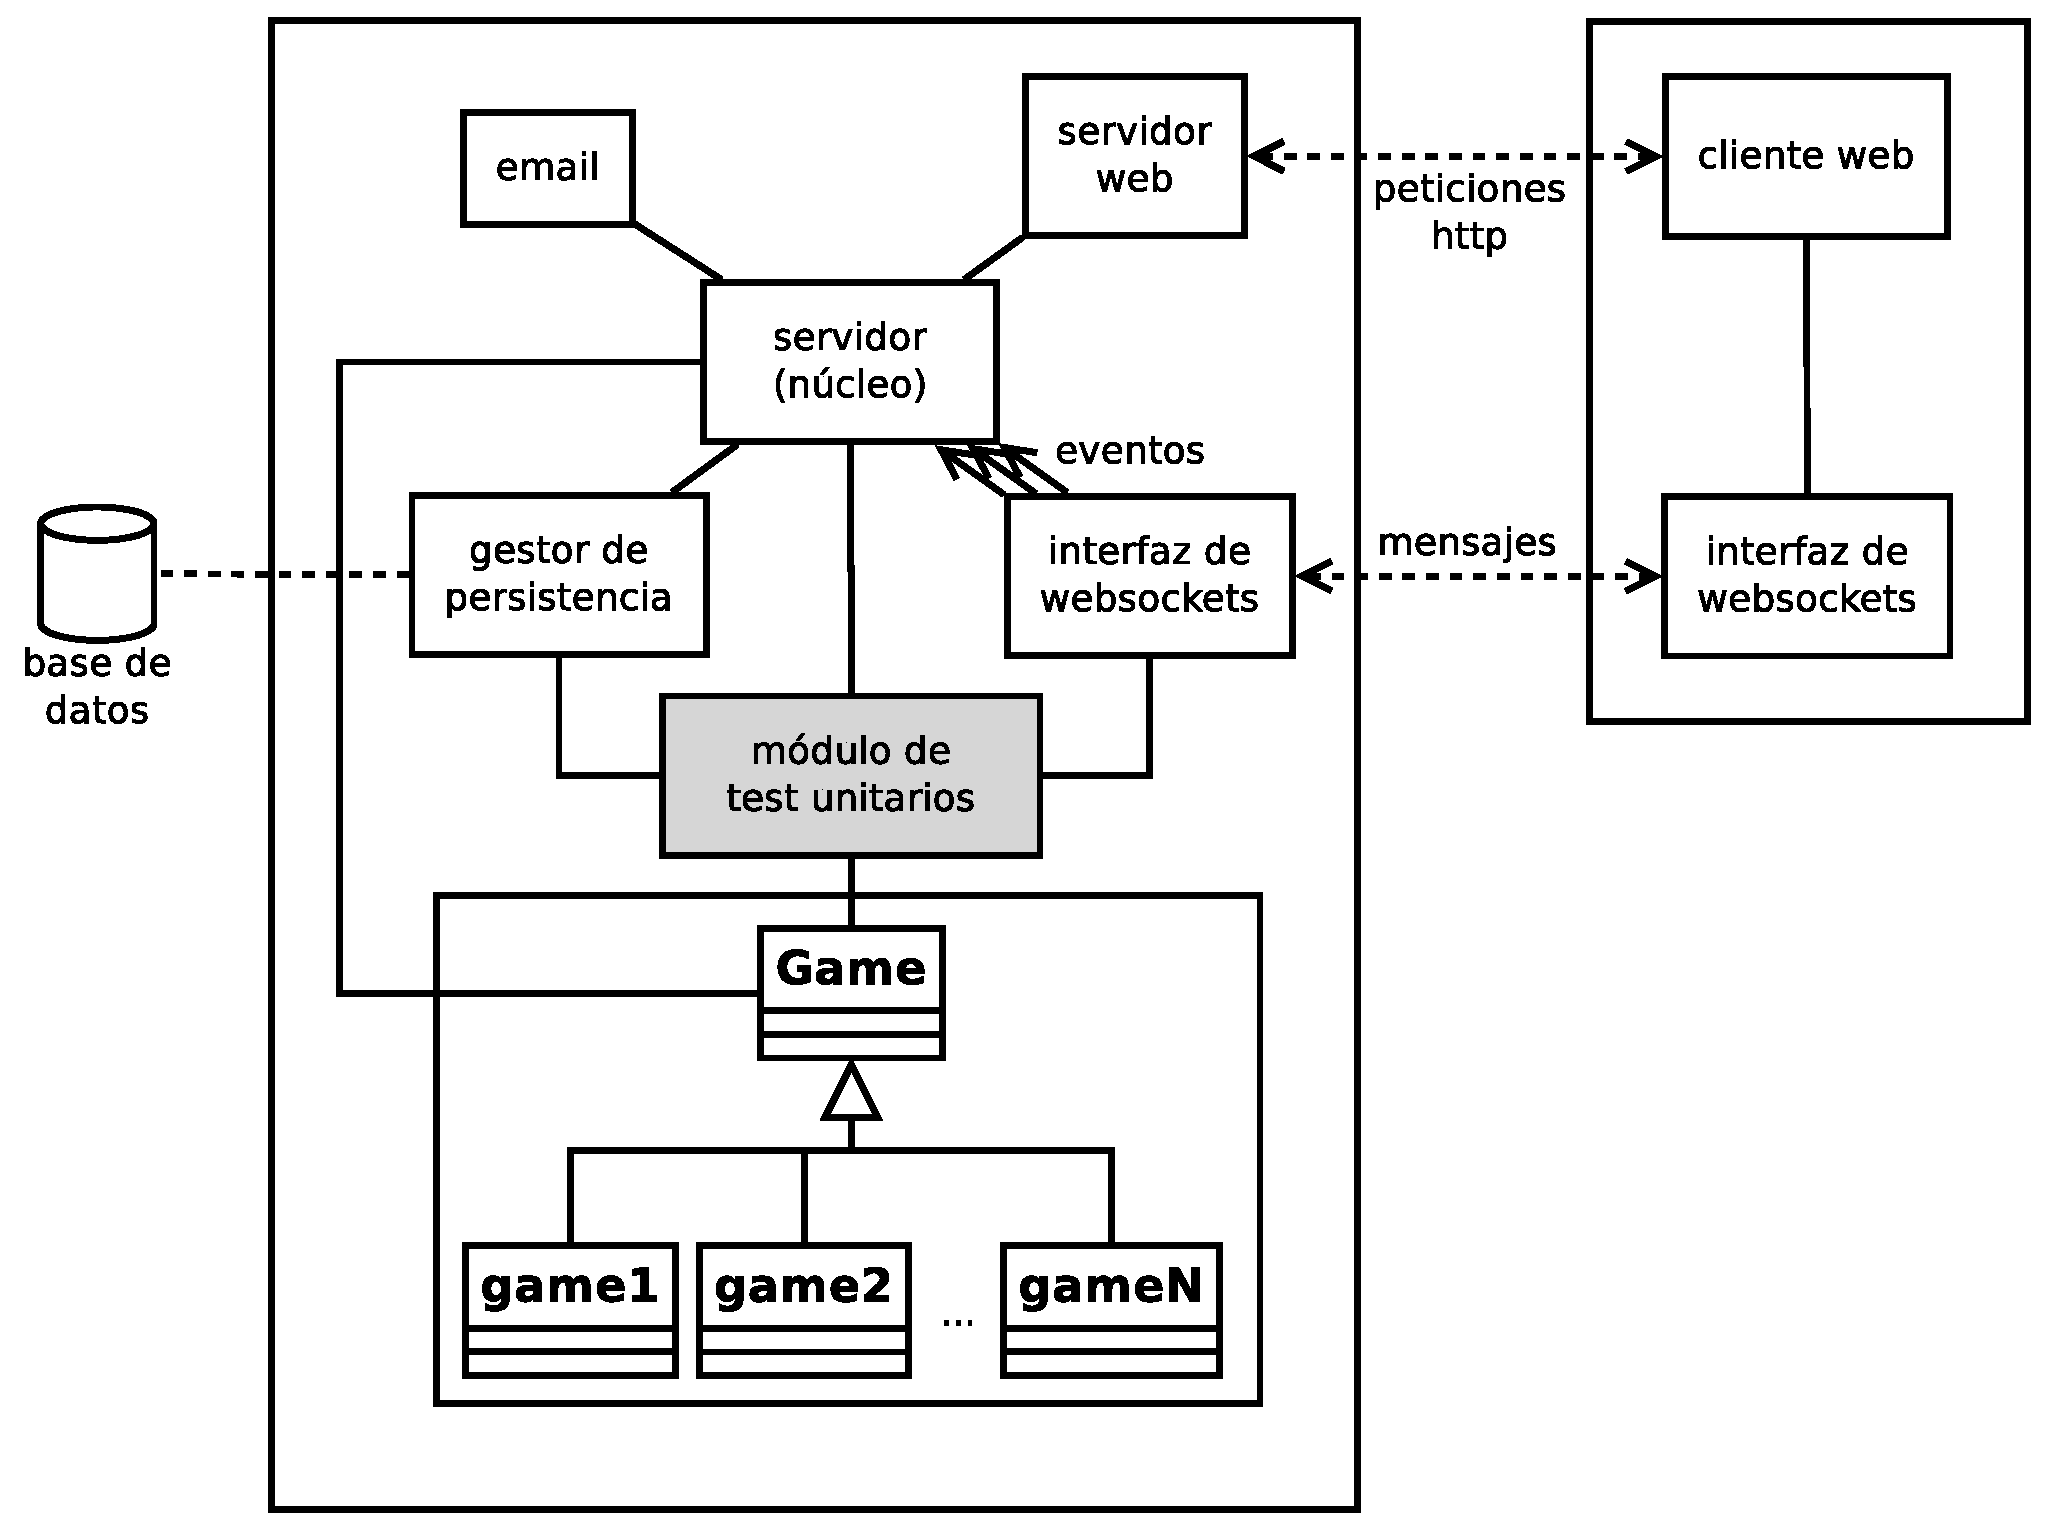
\includegraphics[width=\textwidth]{images/diseno.eps}
    \caption{Diseño modular del sistema}
    \label{fig::diseno}
  \end{center}
\end{figure}

Cada módulo, así como cada capa, ofrece un acoplamiento mínimo con el resto, de tal forma que los cambios efectuados en cualquiera de ellos no afectan directamente a los demás. Por tanto, resulta sencilla la sustitución de módulos por nuevas versiones, por ejemplo, siempre y cuando se respete la interfaz de comunicación.

La figura \ref{fig::diseno} muestra de forma sencilla los componentes que constituyen el sistema, así como la conexión entre ellos. 

\section{Implementación}
\label{sec::implementacion}

La implementación de BreakBrain se ha llevado a cabo completamente desde cero, construyendo una red social completa sin emplear frameworks externos u otras facilidades. Las razones para hacerlo así son diversas, pero la más importante ha sido la voluntad de aprender cómo funciona hasta el más mínimo aspecto de un sistema tan grande y de estas características. Además se decidió apostar por tecnologías muy modernas y con buenos resultados.

En esta sección se presentan brevemente las tecnologías empleadas para implementar el sistema. Posteriormente se analiza la estructura del código fuente escrito, así como pequeñas estadísticas sobre el mismo.

\subsection{Tecnología}

A la hora de analizar las tecnologías empleadas en la construcción de BreakBrain, podemos realizar una sencilla clasificación por el ámbito en el cual han sido empleadas. Así pues, a continuación se detallan los lenguajes de programación, frameworks y entornos de ejecución utilizados por el sistema, y clasificados en tres grupos: servidor, cliente y comunicación.


\subsubsection{Tecnologías del servidor}

\begin{itemize}
\item {\bf JavaScript}: Es el lenguaje empleado para la implementación de todos los componentes del servidor.
\item {\bf NodeJS}: Entorno de ejecución de JavaScript basado en el motor V8 desarrollado por Google. Supone cierta revolución en el ámbito del desarrollo de aplicaciones web de tiempo real.
%\item {\bf Nodester}: \acf{PAAS} de hosting para aplicaciones web implementadas con NodeJS.
\item {\bf Express.js\index{express.js} \cite{Visionmedia}}: framework MVC para el desarrollo de aplicaciones web con NodeJS\index{nodejs}.
\item {\bf MongoDB}:Se trata de un motor de base de datos NoSQL de gran auge en la actualidad. Ofrece muy buenas estadísticas de rendimiento y escalabilidad.
%\item {\bf MongoLab}: \acf{SAAS} de bases de datos MongoDB.
%\item {\bf Amazon Web Storage}: \acf{SAAS} de almacenamiento en la nube.
\end{itemize}


\subsubsection{Tecnologías del cliente}

\begin{itemize}
\item {\bf HTML5}: Tecnología empleada para la construcción del documento estructurado que constituye la interfaz gráfica del cliente: la web.
\item {\bf CSS3}: Hojas de estilos para mejorar la apariencia y comportamiento de los documentos HTML.
\item {\bf JavaScript}: Lenguaje empleado para la implementación del comportamiento de la interfaz gráfica y de la lógica del cliente.
\end{itemize}

\subsubsection{Tecnologías de comunicación}

\begin{itemize}
\item {\bf Websockets}\index{websockets}: Tecnología que proporciona un canal de comunicación bidireccional y full-duplex sobre un único socket TCP. Está diseñada para ser implementada en navegadores y servidores web.
\end{itemize}


\subsection{Estructura del código fuente}

El código fuente está categorizado en dos grandes grupos: el código fuente del servidor y el código fuente del cliente. Dado que todos los lenguajes empleados en el desarrollo son interpretados, no es necesario pensar en procesos de compilación ni archivos binarios.

Para hacer uso de la web cliente, el usuario accede mediante su navegador web a la dirección donde se aloja BreakBrain. Además, las tecnologías empleadas para desarrollar el sistema son estándares soportados por todos los navegadores web modernos. Por tanto, no debemos preocuparnos por ningún tipo de proceso de instalación por parte del usuario. Así mismo, todos los ficheros fuente de BreakBrain se encuentran centralizados en el servidor, por lo que la actualización, corrección de errores, etc. resulta muy sencilla.

El código fuente se encuentra clasificado en la siguiente jerarquía de directorios:

\begin{verbatim}
/                        // Raíz del código. Servidor principal y tests
/node_modules/           // Módulos de terceros para NodeJS 
/server/                 // Módulos de BreakBrain para NodeJS
/server/games/           // Juegos de BreakBrain (parte del servidor)
/server/public/          // Contenido estático servido al cliente
/server/public/games/    // Juegos de BreakBrain (parte publica)
/server/public/js/       // Archivos JavaScript para la web del cliente
/server/public/css/      // Hojas de estilos para la web del cliente
/server/public/img/      // Imágenes servidas para la web del cliente
\end{verbatim}

En el cuadro \ref{tab::code} se ofrece una lista con los diferentes archivos fuente del sistema, junto a una descripción y una muestra de la extensión de cada uno.

\begin{table}
  \caption{Archivos de código fuente}
\label{tab::code}
  \begin{tabular}{lccl}
    \hline
    \tabheadformat
    Fichero fuente & Tipo & Num. de líneas & Descripción \\
    \hline
    {\tt /generator.js} & JavaScript & c & Generador de datos aleatorios \\
    {\tt /server.js} & JavaScript & c & Servidor principal \\
    {\tt /test.js} & JavaScript & c & Módulo de test unitarios \\
    {\tt /test-functionality.js} & JavaScript & c & Batería de tests funcionales \\
    {\tt /test-stress} & JavaScript & c & Batería de tests de estrés \\
    {\tt /server/constants.js} & JavaScript & c & Constantes del programa \\
    {\tt /server/database.js} & JavaScript & c & Módulo de persistencia \\
    {\tt /server/email.js} & JavaScript & c & Módulo de email \\
    {\tt /server/Game.js} & JavaScript & c & ``Clase'' padre de los juegos \\
    {\tt /server/games.js} & JavaScript & c & Módulo servidor de juegos \\
    {\tt /server/util.js} & JavaScript & c & Módulo de utilidades \\
    {\tt /public/games.html} & HTML & c & d \\
    {\tt /public/header.html} & HTML & c & d \\
    {\tt /public/home.html} & HTML & c & d \\
    {\tt /public/login.html} & HTML & c & d \\
    {\tt /public/logout.html} & HTML & c & d \\
    {\tt /public/password.html} & HTML & c & d \\
    {\tt /public/people.html} & HTML & c & d \\
    {\tt /public/profile.html} & HTML & c & d \\
    {\tt /public/css/*} & CSS & c & Hojas de estilos del cliente \\
    {\tt /public/js/*} & JavaScript & c & Archivos JavaScript del cliente \\
    \hline
  \end{tabular}

  
\end{table}


\section{Estadísticas del código fuente}

En el cuadro \ref{tab::stat} se muestra el nivel de utilización de cada lenguaje ---de programación o maquetación--- en la implementación de BreakBrain. Nótese la diferenciación entre JavaScript del lado del cliente y JavaScript del lado del servidor. Se ha realizado esta separación por la naturaleza clásica del desarrollo web de emplear dos lenguajes diferentes para el cliente y el servidor. En este caso se trata del mismo lenguaje, pero resulta de interés realizar una comparativa de la cantidad de código escrito en ambos extremos de la comunicación.

\begin{table}
  \caption{Estadísticas del código fuente de BreakBrain}
  \label{tab::stat}

  \begin{center}   
  \begin{tabular}{cccc}
    \hline
    \tabheadformat
    Lenguaje & Nº de archivos & Líneas de código & Protagonismo \\
    \hline
    JavaScript (cliente) & & & \\
    JavaScript (servidor) & & & \\
    HTML5 & & & \\
    CSS3 & & & \\
    \hline
  \end{tabular}
  \end{center}
\end{table}



\section{Pruebas}

Con el fin de asegurar la calidad del software construido se han llevado a cabo diferentes tipos de pruebas sobre el mismo.

\subsection{Pruebas unitarias}

Para la realización de las pruebas unitarias se ha desarrollado un pequeño módulo ({\tt test.js}), que permite la realización de tests sencillos. Estos tests se han repartido por el código fuente en los puntos donde semánticamente tienen sentido, y sólo se lanzan si al ejecutar el servidor se le añade el argumento {\tt -t}. Al ejecutar el servidor de esta forma, el log muestra los casos de éxito y fracaso de todos los tests unitarios. Al finalizar los mismos se ofrece una pequeña estadística del resultado obtenido.

El subsistema de test tiene la particularidad de que posibilita su uso desde los nuevos juegos que se creen, ofreciendo así una manera sencilla de realizar tests unitarios desde la implementación del nuevo juego sin tener que utilizar otros módulos externos. La forma de llevar a cabo tests es muy sencilla:

\begin{verbatim}
test('descripción del test', 
      expresion_que_debe_ser_true, // por ejemplo: instancia != null
     'mensaje de error');
\end{verbatim}

El resultado de la ejecución de los tests unitarios básicos del sistema es la mostrada en la figura \ref{fig::unit}. Nótese que dicho resultado es el correspondiente al caso de ejecución más básico, en el que no se carga ningún juego, por lo que a medida que se carguen diferentes juegos dotados de tests, esta salida será mayor.

\begin{figure}[h]
  \begin{center}
    
    \begin{verbatim}
sgmonda@envy:~/projects/breakbrain $ node server.js -t
27 Nov 2012 19:24:30::UNIT TEST 1 CORRECT: constants module load
27 Nov 2012 19:24:30::DATABASE: Connecting to MongoDB database...
27 Nov 2012 19:24:30::UNIT TEST 2 CORRECT: mongodb module load
27 Nov 2012 19:24:30::UNIT TEST 3 CORRECT: database server creation
27 Nov 2012 19:24:30::UNIT TEST 4 CORRECT: database object creation
27 Nov 2012 19:24:30::UNIT TEST 5 CORRECT: database collection retrieval
27 Nov 2012 19:24:30::UNIT TEST 6 CORRECT: connection to mongo server
27 Nov 2012 19:24:30::UNIT TEST 7 CORRECT: connection to mongo db
27 Nov 2012 19:24:31::UNIT TEST 8 CORRECT: database connection opening
27 Nov 2012 19:24:32::UNIT TEST 9 CORRECT: database authentication
27 Nov 2012 19:24:32::DATABASE: Connected and authenticated successfully
27 Nov 2012 19:24:32::UNIT TEST 10 CORRECT: database object instantiation
27 Nov 2012 19:24:32::UNIT TEST 11 CORRECT: fs module load
27 Nov 2012 19:24:32::UNIT TEST 12 CORRECT: express module load
27 Nov 2012 19:24:32::UNIT TEST 13 CORRECT: http module load
27 Nov 2012 19:24:32::UNIT TEST 14 CORRECT: web app creation
27 Nov 2012 19:24:32::EMAIL-MODULE: Email subsystem ready to send emails
27 Nov 2012 19:24:32::UNIT TEST 15 CORRECT: email module load
27 Nov 2012 19:24:32::GAMES-MODULE: Loading games server...
27 Nov 2012 19:24:32::WEB SERVER: running on port 20661
27 Nov 2012 19:24:32::UNIT TEST 16 CORRECT: games directory reading
27 Nov 2012 19:24:32::UNIT TEST 17 CORRECT: games count
27 Nov 2012 19:24:32::GAMES-MODULE: Loading game "Un juego"...
27 Nov 2012 19:24:32::UNIT TEST 18 CORRECT: particular game load
27 Nov 2012 19:24:32::UNIT TEST 19 CORRECT: games module load
27 Nov 2012 19:24:32::UNIT TEST 20 CORRECT: websockets module load
27 Nov 2012 19:24:32::WEBSOCKETS SERVER: running on port 20661
27 Nov 2012 19:24:32::MAIN SERVER: The whole server is ready!

27 Nov 2012 19:24:32::CORRECT UNIT TESTS: 20 (100%)
^Csgmonda@envy:~/projects/breakbrain $ 

    \end{verbatim}

    \caption{Resultado parcial de tests unitarios}
    \label{fig::unit}
  \end{center}
\end{figure}


\subsection{Pruebas funcionales}

Se han llevado a cabo una serie de pruebas funcionales automatizadas, que cubren los aspectos más importantes de la funcionalidad especificada en los apartados \ref{sec::requisitos} y \ref{sec::casos}. Dada la naturaleza asíncrona y no bloqueante de la tecnología con la que ha sido desarrollado el servidor del proyecto, estas pruebas se lanzan y analizan de forma asíncrona. Para ello se ha utilizado un módulo de NodeJS\index{nodejs} llamado \emph{Vows} \cite{Maecki}\index{vows}.

Estas pruebas se encuentran en el archivo {\tt tests-functionality.js}, y pueden lanzarse sobre el intérprete de NodeJS\index{nodejs} una vez que el servidor está en ejecución. Los resultados de estas pruebas se muestran en la figura \ref{fig::vows}.

\begin{figure}[h]
  \begin{center}
    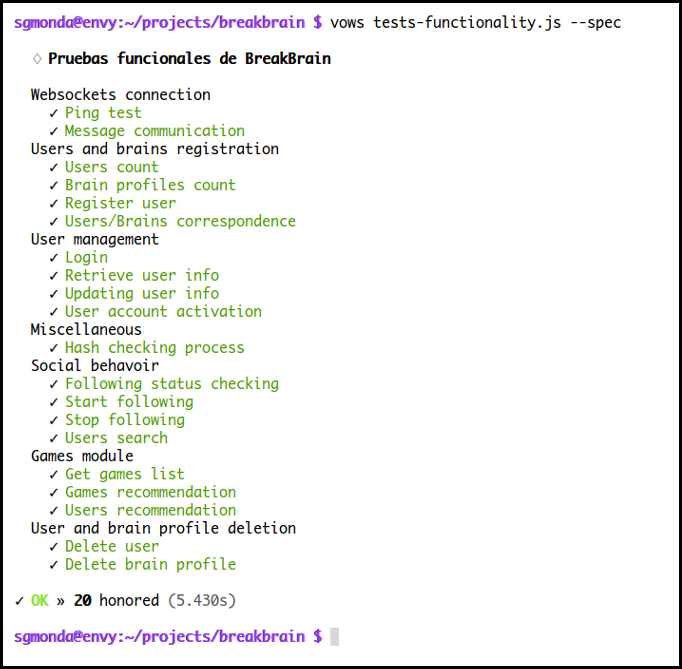
\includegraphics[width=0.8\textwidth]{images/vows.png}
    \caption{Resultados de la batería de tests funcionales}
    \label{fig::vows}
  \end{center}
\end{figure}



\subsection{Pruebas de aceptación}

Durante el desarrollo del sistema se han realizado pequeñas y repetidas pruebas de aceptación por parte de un subconjunto variado de usuarios finales, recogiendo las opiniones de los mismos y empleando éstas, junto con las estadísticas obtenidas, para la corrección de errores y mejora de aspectos varios.

La elección del subconjunto poblacional sometido a las pruebas de aceptación se ha llevado a cabo mediante un muestreo aleatorio estratificado, con el objetivo de obtener opiniones y observaciones de uso de usuarios de diferentes edades. Los estratos definidos para la realización del muestreo son los siguientes:

\begin{itemize}
\item Joven (entre 15 y 30 años de edad)
\item Adulto 1 (entre 30 y 45 años de edad)
\item Adulto 2 (entre 45 y 60 años de edad)
\end{itemize}

Durante la planificación de las pruebas se seleccionó aleatoriamente un individuo de cada subconjunto ---dichas personas se comprometieron a someterse a las pruebas de forma periódica---. Los individuos representantes de cada estrato son los siguientes:

\begin{itemize}
\item Joven - Rodrigo Testillano
\item Adulto 1 - Néstor Ceballos
\item Adulto 2 - Rafael García
\end{itemize}


En total se han llevado a cabo 3 sesiones de pruebas de aceptación. A continuación se enumeran las actividades en las que consistió cada una de ellas:

\renewcommand{\labelenumi}{\bf PA-\arabic{enumi}}
\renewcommand{\labelenumii}{\arabic{enumii}. }
\begin{enumerate}
\item La primera sesión consistió en:
  \begin{itemize}
  \item Crearse una cuenta en la red social.
  \item Autenticarse en el sistema.
  \item Cerrar la sesión.
  \item Tratar de acceder al sistema con datos erróneos.
  \item Simular el olvido de la contraseña para recuperar el acceso a su cuenta.
  \end{itemize}

\item La segunda sesión comprendió el uso de la red y la gestión de perfiles:
  \begin{enumerate}
  \item Explorar las estadísticas del perfil de usuario.
  \item Modificar la información personal del perfil.
  \item Modificar las preferencias de entrenamiento cerebral.
  \item Búsqueda de usuarios.
  \item Seguir y dejar de seguir a otros usuarios.
  \end{enumerate}

\item En la tercera sesión los individuos utilizaron el subsistema de juegos: 
  \begin{enumerate}
  \item Exploración de los juegos individuales.
  \item Exploración de los juegos multijugador.
  \item Jugar a un juego monojugador.
  \item Retar a otro usuario a un juego multijugador.
  \item Ser retado por otro usuario y aceptar. Jugar parida multijugador.
  \item Ser retado por otro usuario y rechazar la invitación.
  \end{enumerate}

\end{enumerate}

Los resultados obtenidos durante estas pruebas de aceptación fueron de gran utilidad, no sólo para solucionar ciertos problemas que no habían sido localizados hasta el momento de la utilización del sistema por parte del usuario final, sino también para mejorar la \emph{usabilidad}\index{usabilidad} ante problemas de diseño detectados durante la observación del uso por parte de los individuos. En resumen, algunos de los beneficios de estas pruebas fueron los siguientes:

\begin{itemize}
\item Corrección de pequeños errores de programación (\emph{bugs}\index{bug}).
\item Corrección de problemas de distribución de elementos en la web (problemas de usabilidad\index{usabilidad}).
\item Aceptación de críticas sobre los esquemas de color y rediseño de los mismos.
\item Mejora de la interacción hombre-máquina ante la observación de dificultades de uso de algunos componentes por parte de ciertos individuos.
\end{itemize}


\subsection{Pruebas de estrés del sistema}

Esta batería de pruebas permite observar el comportamiento y escalabilidad del sistema, observando el comportamiento del mismo en situaciones de poca carga y en situaciones extremas, con gran cantidad de peticiones costosas simultáneas.

Cabe añadir que la probabilidad de que el sistema se vea sometido a estas situaciones extremas en un entorno real es despreciable. Sin embargo, estas pruebas resultan de gran utilidad para estudiar la respuesta del servidor y la base de datos.

\begin{figure}[h]
  \begin{center}
    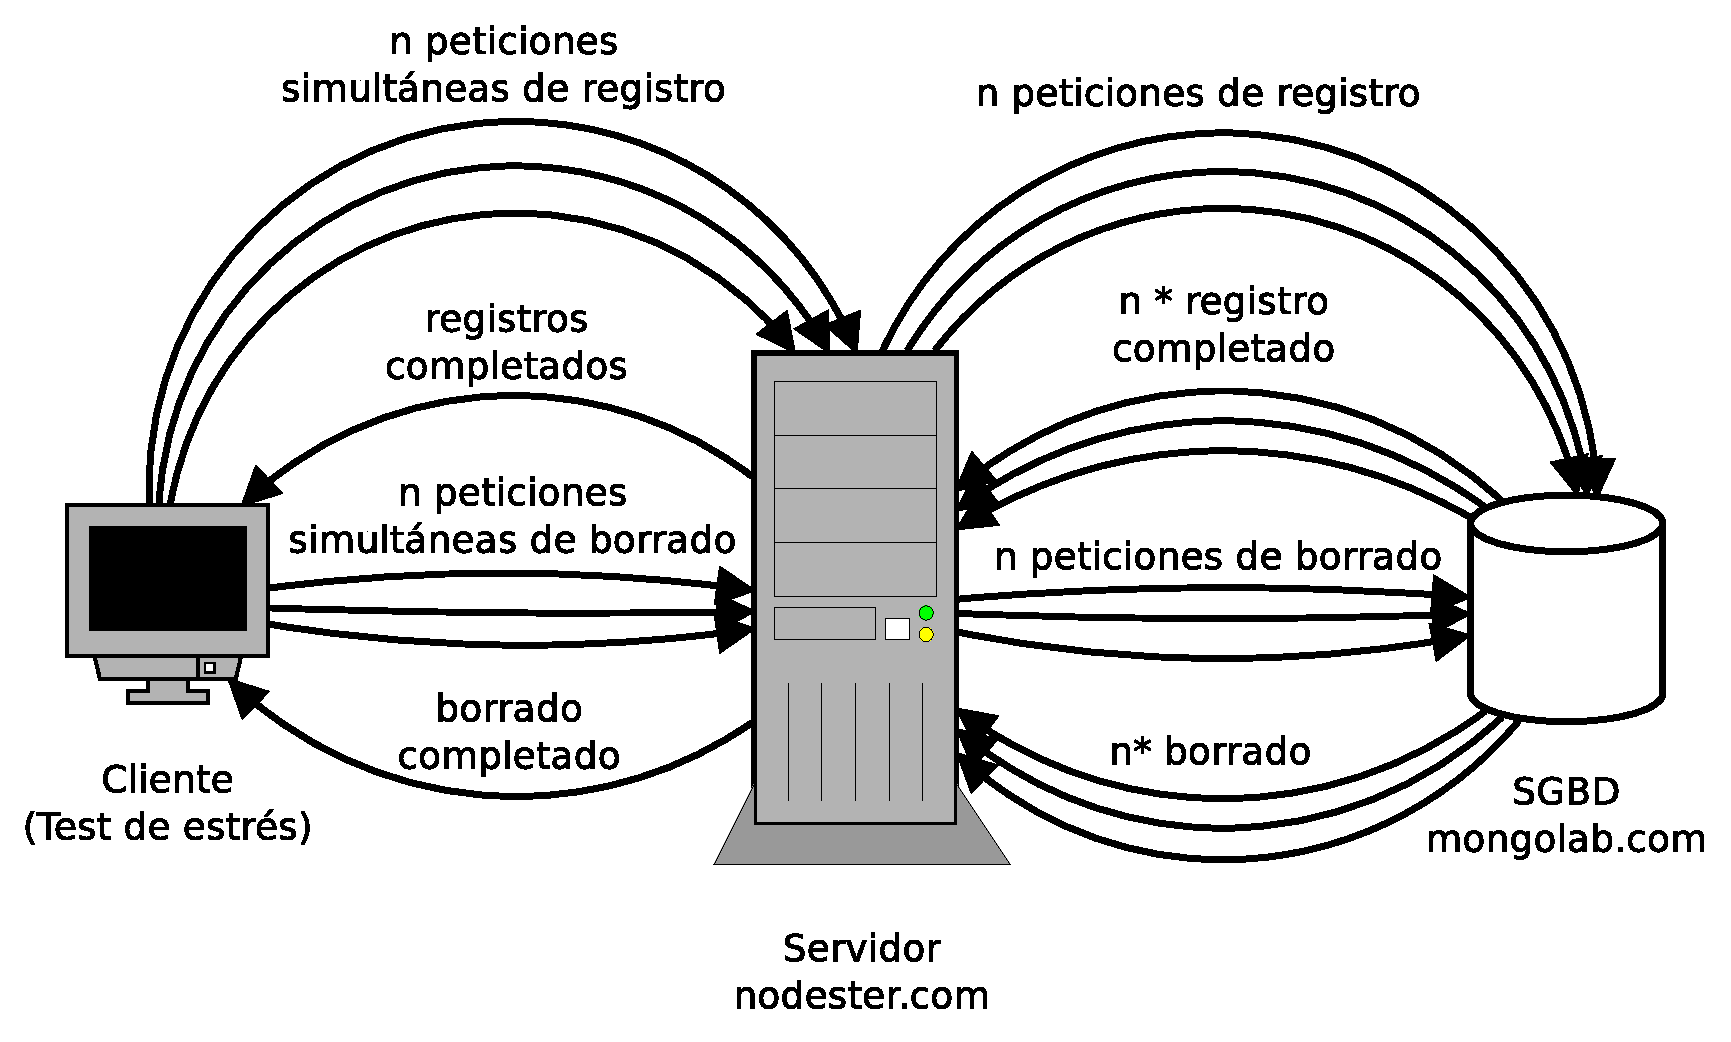
\includegraphics[width=\textwidth]{images/estres.eps}
    \caption{Diseño del test de estrés}
    \label{fig::estres}
  \end{center}
\end{figure}

Para realizar las pruebas de estrés se ha diseñado un pequeño programa que lanza peticiones simultáneas contra el servidor. Las peticiones lanzadas son de registro y borrado de usuarios. Se ha seleccionado la operación de registro de un usuario ---con generación aleatoria de datos--- porque es la que más coste tiene para la base de datos, y así nos permite abarcar toda la amplitud del sistema. Por otro lado, las operaciones de eliminación se han incluido en el test símplemente para eliminar los usuarios y perfiles cerebrales creados en la etapa anterior, y así servir también de contraste, al tratarse de la operación de menor coste de la base de datos.

Los resultados obtenidos son los siguientes:

\begin{itemize}
\item 1 única petición (RAM: 13MB)

  \begin{lstlisting}
STRESS-TEST: Starting stress test
STRESS-TEST: 1 false users registered
Time spent in 1 false users registration: 648ms
STRESS-TEST: False users deleted
STRESS-TEST: Stress test finished in 
Time spent in 1 false users deletion: 270ms
Time spent in whole stress test: 918ms
  \end{lstlisting}
  

\item 10 peticiones simultáneas (RAM: 15.7MB)
  \begin{lstlisting}
STRESS-TEST: Starting stress test
STRESS-TEST: 10 false users registered
Time spent in 10 false users registration: 964ms
STRESS-TEST: False users deleted
STRESS-TEST: Stress test finished in 
Time spent in 10 false users deletion: 272ms
Time spent in whole stress test: 1236ms
  \end{lstlisting}

\item 20 peticiones simultáneas (RAM: 17MB)
  \begin{lstlisting}
STRESS-TEST: Starting stress test
STRESS-TEST: 20 false users registered
Time spent in 20 false users registration: 469ms
STRESS-TEST: False users deleted
STRESS-TEST: Stress test finished in 
Time spent in 20 false users deletion: 277ms
Time spent in whole stress test: 748ms
  \end{lstlisting}

\item 50 peticiones simultáneas (RAM: 19MB)
  \begin{lstlisting}
STRESS-TEST: Starting stress test
STRESS-TEST: 50 false users registered
Time spent in 50 false users registration: 864ms
STRESS-TEST: False users deleted
STRESS-TEST: Stress test finished in 
Time spent in 50 false users deletion: 320ms
Time spent in whole stress test: 1186ms
  \end{lstlisting}

\item 100 peticiones simultáneas (RAM: 21.4MB)
  \begin{lstlisting}
STRESS-TEST: Starting stress test
STRESS-TEST: 100 false users registered
Time spent in 100 false users registration: 6955ms
STRESS-TEST: False users deleted
STRESS-TEST: Stress test finished in 
Time spent in 100 false users deletion: 1387ms
Time spent in whole stress test: 8342ms
  \end{lstlisting}

\item 200 peticiones simultáneas (RAM: 28.5MB)
  \begin{lstlisting}
STRESS-TEST: Starting stress test
STRESS-TEST: 200 false users registered
Time spent in 200 false users registration: 14460ms
STRESS-TEST: False users deleted
STRESS-TEST: Stress test finished in 
Time spent in 200 false users deletion: 1870ms
Time spent in whole stress test: 16330ms
  \end{lstlisting}

\item 500 peticiones simultáneas (RAM: 59MB)
  \begin{lstlisting}
STRESS-TEST: Starting stress test
STRESS-TEST: 500 false users registered
Time spent in 500 false users registration: 34901ms
STRESS-TEST: False users deleted
STRESS-TEST: Stress test finished in 
Time spent in 500 false users deletion: 5654ms
Time spent in whole stress test: 40555ms
  \end{lstlisting}

\item 1000 peticiones simultáneas (RAM: 128MB)
  \begin{lstlisting}
STRESS-TEST: Starting stress test
STRESS-TEST: 1000 false users registered
Time spent in 1000 false users registration: 65909ms
STRESS-TEST: False users deleted
STRESS-TEST: Stress test finished in 
Time spent in 1000 false users deletion: 14254ms
Time spent in whole stress test: 80163ms
  \end{lstlisting}

\item 5000 peticiones simultáneas (RAM: 340MB)
  \begin{lstlisting}
STRESS-TEST: Starting stress test
STRESS-TEST: 5000 false users registered
Time spent in 5000 false users registration: 322281ms
STRESS-TEST: False users deleted
STRESS-TEST: Stress test finished in 
Time spent in 5000 false users deletion: 75101ms
Time spent in whole stress test: 397382ms
  \end{lstlisting}

\item 10000 peticiones simultáneas (RAM: 520MB)
  \begin{lstlisting}
STRESS-TEST: Starting stress test
STRESS-TEST: 10000 false users registered
Time spent in 10000 false users registration: 547662ms
STRESS-TEST: False users deleted
STRESS-TEST: Stress test finished in 
Time spent in 10000 false users deletion: 229148ms
Time spent in whole stress test: 776810ms
  \end{lstlisting}

\end{itemize}

\begin{table}
  \caption{Estadísticas de las pruebas de estrés en un servidor Debian 64-bits Linux 3.2.0, CPU Intel Core i7 Q720 1.60GHz x 4, RAM 6GB}
  \begin{center}   
    \begin{tabular}{|c||c|c|c||c|}
      \hline
      \tabheadformat
      Peticiones & Tiempo total de & Tiempo total de & Tiempo total & Memoria RAM\\
     \tabheadformat
      simultáneas & inserciones & eliminaciones & del test & (server)\\
      \hline      \hline
      1 & 669 ms & 271 ms & 940 ms & 13 MB\\
      \hline
      10 & 964 ms & 272 & 1236 ms & 15.7 MB\\
      \hline
      20 & 469 ms & 277 ms & 748 ms & 17 MB\\
      \hline
      50 & 864 ms & 320 ms & 1186 ms & 19 MB\\
      \hline
      100 & 6955 ms & 1387 ms & 8342 ms & 21.4 MB\\
      \hline
      200 & 14460 ms & 1870 ms & 16330 ms & 28.5 MB\\
      \hline
      500 & 34901 ms & 5654 ms & 40555 ms & 50 MB\\
      \hline
      1000 & 65909 ms & 14254 ms & 80163 ms & 128 MB\\
      \hline
      5000 & 322281 ms & 75101 ms & 397382 ms & 340 MB\\
      \hline
      10000 & 547662 ms & 229148 ms & 776810 ms & 520 MB\\
      \hline
    \end{tabular}
  \end{center}
\end{table}


\begin{figure}[h]
  \begin{center}
    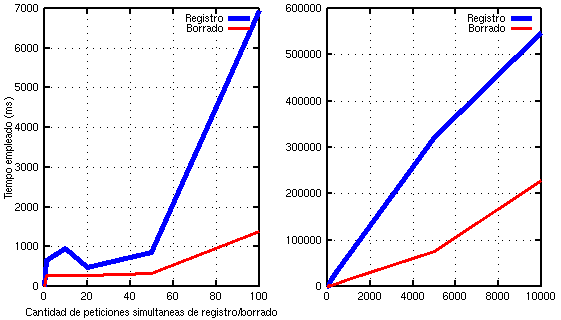
\includegraphics[width=\textwidth]{images/estresplot.png}
    \caption{Resultados de las pruebas de estrés}
    \label{fig::estres-plot}
  \end{center}
\end{figure}

A la vista de los resultados puede observarse el buen comportamiento del servidor para situaciones normales y extremas. Por supuesto, el caso de recibir gran cantidad de peticiones de registro simultáneas es muy poco probable, pero nos da una idea del rendimiento del sistema. El registro es la operación más costosa (para el subsistema de base de datos), y por ello ha sido elegida como \emph{operación estresante} para someter al sistema a ella.


% function drawVisualization() {
%   // Create and populate the data table.
%   var data = google.visualization.arrayToDataTable([
%     ['x', 'Registro', 'Borrado', 'RAM'],
%     ['0',   0,       0,           20.5],
%     ['1',   669,       271,         1],
%     ['10',   964,       272,           0.5],
%     ['20',   469,       277,         1],
%     ['50',   864,       320,           0.5],
%     ['100',   6955,       1387,         1],
%     ['200',   14460,       1870,           0.5],
%     ['500',   34901,       5654,         1],
%     ['1000',   65909,       14254,           0.5],
%     ['5000',   65909,       14254,           0.5],
%     ['10000',   65909,       14254,           0.5],
%     ['50000',   65909,       14254,           0.5]
%   ]);

%   // Create and draw the visualization.
%   new google.visualization.LineChart(document.getElementById('visualization')).
%       draw(data, {curveType: "function",
%                   width: 500, height: 400,
%                   vAxis: {maxValue: 10}}
%           );
% }
% ​



